\documentclass{report}

% ============ PACKAGES ============= %
\usepackage[dutch]{babel}
\usepackage[margin=3cm]{geometry}
\usepackage{fancyhdr}
\usepackage{eso-pic}
\usepackage{setspace}
\usepackage{titlesec}
\usepackage{xcolor}

\usepackage{amsmath}
\usepackage{amsfonts}
\usepackage{amssymb}
\usepackage{gensymb}

\usepackage{graphicx}
\usepackage{subfigure}
\usepackage{float}

\usepackage{hyperref}
\usepackage{cite}

% ============ METADATA ============= %
\title{Toepassing van neurale netwerken voor een accurate karakterisatie van de chemische samenstelling van nanodeeltjes met energie-dispersieve X-stralenspectroscopie}
\author{Wouter Heyvaert}

\makeatletter
\let\Title\@title
\let\Author\@author
\let\Date\@date
\makeatother

% ============= LAYOUT ============== %
\pagestyle{fancy}
\fancyhead{}
\renewcommand{\chaptermark}[1]{\markboth{#1}{}}
\fancyhead[R]{\thechapter\ \MakeUppercase{\leftmark}}

\hypersetup{
    colorlinks=true,
    bookmarks=true,
    linkcolor=[RGB]{114,17,41},
    urlcolor=[RGB]{114,17,41},
    citecolor=red,
}

\newcommand{\BackgroundPic}{
	\put(0,0){
		\parbox[b][\paperheight]{\paperwidth}{
			\centering
			\includegraphics[width=\paperwidth,keepaspectratio]{ua_logo.pdf}
		}
	}
}

\titleformat{\chapter}{\normalfont\bfseries}{\Huge\thechapter}{1em}{\Huge}

\definecolor{accent}{RGB}{114,17,41}

% ============ DOCUMENT ============= %
\begin{document}

\begin{titlepage}

	\centering
	\includegraphics[width=7cm,keepaspectratio]{ua_logo.png}\\[1.5cm]
	\LARGE\textsc{Universiteit Antwerpen}\\[0.2cm]
	\LARGE\textsc{Faculteit Wetenschappen}\\[1cm]
	\LARGE\textsc{\color{accent}Bachelorproef Fysica}\\[0.2cm]
	
	\rule{\linewidth}{0.5mm}\\
	\huge\textbf{\Title}
	\rule{\linewidth}{0.5mm}\\[0.5cm]
	
	\begin{minipage}[t]{0.4\textwidth}
	\begin{flushleft}\large
	\text{Auteur:}\\
	{\color{accent}Wouter Heyvaert}
	\end{flushleft}
	\end{minipage}
	~
	\begin{minipage}[t]{0.4\textwidth}
	\begin{flushright}\large
	\text{Promotor:} \\
	{\color{accent}Prof. Dr. Sara Bals}\\[0.2cm]
	\text{Onderzoeksgroep:}\\
	{\color{accent}Elektronenmicroscopie voor materiaalonderzoek}\\[0.2cm]
	\text{Begeleiders:} \\
	{\color{accent}Alexander Skorikov\\Hans Vanrompay}
	\end{flushright}
	\end{minipage}\\[2cm]
	
	\Large\textsc{Academiejaar 2019-2020}

\end{titlepage}


\chapter*{Abstract}
Since many years, the scientific interest in the world of nanomaterials has been increasing. This is because nanomaterials often have characteristics that cannot be found in macroscopic materials, caused by the increased importance of surface electrons and quantum effects. For example, nanoparticles interact strongly with visible light due to surface plasmon resonance. Therefore, it shouldn't be a surprise that many applications using nanomaterials have been made available and are still being investigated. However, to use nanomaterials at their best, it is crucial to gain better understandings about the relations between their shape, chemical composition and properties. This information can then be used to aid in the synthesis of nanoparticles with predefined properties. Transmission electron microscopy (TEM) has been an invaluable tool for gaining information about the shape and composition of such nanomaterials. Their shape can be studied by combining electron microscopy with tomography. This is a powerful technique to reconstruct the three-dimensional (3D) shape by analyzing a series of two-dimensional (2D) projection images from a range of different angles. However, when a nanoparticle is composed out of seperate elements, it is also important to gain knowledge about the influence of its 3D chemical composition on its properties. To do this, one can use the Z-contrast present in HAADF-STEM (high-angle annular dark-field scanning transmission electron microscopy) projection images. Namely, when the different elements have Z-values that are significantly distinctive, and when the different elements are spatially seperated from each other, there will be contrast in the intensities from voxels corresponding to seperate elements in the 3D reconstruction from a HAADF-STEM tilt series. But if one of both conditions is not met, other methods are required.
\\ \\
Energy-dispersive X-ray spectroscopy (EDX) makes it possible to investigate the presence of each element in a nanomaterial seperately. By combining EDX with tomography, it is then possible to investigate the 3D spatial distribution of different elements throughout the nanoparticle. However, EDX maps typically have a very low signal-to-noise ratio. Therefore extended measurement times are often necessary for an accurate characterisation. On the other hand, excessive measurement times are impractical, since long exposure to the electron beam damages the nanoparticles. Moreover, tomography requires multiple projection images taken from different angles. This puts a limit on the measurement time per angle, and thus on the signal-to-noise ratio. The accuracy of tomography declines whenever the projection images are deteriorated by high amounts of noise, causing a need for noise reduction in post processing. A gaussian filter is a common choice for this task. In this thesis I will investigate the use of artificial neural networks for improving this noise reduction post-processing step, thus the accuracy of EDX tomography. These networks have the advantage that they can gather prior knowledge about the data during their training process, making them better suitable for noise reduction than classical methods such as a gaussian filter. It will be shown that noise reduction with a neural network yields more accurate results when studying EDX maps with a low signal-to-noise ratio. Furthermore, the power of denoising with neural networks will be used to show that a more accurate 3D reconstruction can be achieved from EDX tomography.


\chapter*{Samenvatting}
Sinds vele jaren is de interesse in de wereld van nanomaterialen sterk toegenomen. Deze materialen hebben vaak eigenschappen die niet terug te vinden zijn bij materialen op grotere schaal. Die eigenschappen worden voornamelijk veroorzaakt door het feit dat oppervlakte elektronen en kwantummechanische effecten een belangrijkere rol spelen bij de kleine afmetingen van nanodeeltjes. Nanodeeltjes interageren bijvoorbeeld sterk met zichtbaar licht omwille van oppervlakte plasmonresonanties. Het is dan ook niet verwonderlijk dat er steeds meer toepassingen van nanomaterialen beschikbaar worden. Om nanomaterialen optimaal te benutten, is het belangrijk om hun kenmerken goed te begrijpen en te kunnen voorspellen. Deze informatie kan dan gebruikt worden om nanomaterialen met specifieke eigenschappen te synthetiseren. Transmissie elektronenmiscroscopie (TEM) is een onmisbaar hulpmiddel om de connectie tussen de vorm, samenstelling en eigenschappen van deze materialen te onderzoeken. De vorm kan men bepalen door tomografie te combineren met projectiebeelden die men in een TEM kan bekomen. Tomografie is een techniek om tweedimensionale (2D) projectiebeelden om te zetten in een driedimensionale (3D) reconstructie. Indien een nanomateriaal gemaakt is van verschillende atoomsoorten, dan is het ook belangrijk om te beschrijven welke invloed de 3D chemische samenstelling van het materiaal heeft op de eigenschappen van dat materiaal. Indien de atoomnummers van de elementen voldoende verschillen met elkaar, en indien de materialen niet met elkaar vermengd zijn, dan is het mogelijk om het Z-contrast van het HAADF-signaal (high-angle annular dark-field) te benutten. Door dit Z-contrast zullen de verschillende elementen overeenkomen met verschillende voxel-intensiteiten in de 3D reconstructie van een tiltreeks van HAADF-STEM (high-angle annular darkfield scanning transmissie elektronenmicroscopie) projectiebeelden. Als aan één van die twee eisen niet voldaan is, dan is een andere methode vereist.
\\ \\
Met energie-dispersieve X-stralen spectroscopie (EDX) is het mogelijk om de aanwezigheid van elk element in een nanomateriaal afzonderlijk te bestuderen. Door EDX te combineren met tomografie is het mogelijk om van elk element afzonderlijk een 3D reconstructie te maken. Echter, EDX maps hebben typisch een zeer lage signaal-ruis verhouding. Dat heeft als gevolg dat er lange meettijden nodig zijn om betrouwbare conclusies te kunnen trekken over de verdeling van de atoomsoorten in het sample. Anderzijds is de meettijd beperkt omdat het sample na een lange blootstelling aan de elektronenbundel beschadigd wordt. Deze lage signaal-ruis verhouding is ook een limiterende factor voor EDX tomografie. Er moet immers een tiltreeks van projectiebeelden onder verschillende invalshoeken opgenomen worden, wat resulteert in een beperkte signaal-ruis verhouding per projectiebeeld. Tomografie is bovendien zeer moeilijk bij grote hoeveelheden ruis, met als gevolg dat de ruis in EDX maps gereduceerd moet worden in naverwerking. Gewoonlijk wordt daarvoor een gaussische filter gebruikt. In deze thesis zal ik onderzoeken of er meer accurate resultaten bekomen kunnen worden door gebruik te maken van artificiële neurale netwerken. Neurale netwerken hebben het voordeel dat ze voorkennis over de data kunnen verkrijgen tijdens het optimalizatieproces van deze netwerken. Dat maakt een meer nauwkeurige ruisvermindering mogelijk. Er zal aangetoond worden dat deze methoden een accurate karakterisatie van de EDX maps toelaten, zelfs als deze een zeer lage signaal-ruis verhouding hebben. Bovendien zal de kracht van ruisvermindering met neurale netwerken gebruikt worden om aan te tonen dat een nauwkeurigere 3D reconstructie mogelijk is met EDX tomografie.


\chapter*{Dankwoord}
Alvorens een diepe duik te nemen in de wereld van nanomaterialen zou ik even de tijd willen nemen om een aantal personen te bedanken. Het werk dat in deze thesis voorgelegd wordt, was zonder hen namelijk niet mogelijk.
\\ \\
Eerst en vooral wil ik mijn promotor, Prof. Dr. Sara Bals, bedanken. Van in het begin stond ze enthousiast klaar met een grote variëteit aan onderwerpen en, hoewel ik zelf niet goed wist aan welk type onderwerp ik het liefst wilde werken, kon ze mij al snel in contact brengen met de juiste personen om deze keuze te kunnen maken. Daarom wil ik ook Alexander Skorikov en Adrian Pedrazo Tardajos bedanken. Zij gaven me vol overtuiging een uitgebreide uitleg over de werking van EMAT en verschillende onderwerpen waaraan ik zou kunnen werken. Ik koos ervoor om samen te werken met Alexander, en hij stond elke dag klaar om mij met raad en daad bij te staan en om samen mijn vooruitgang te bespreken. De vele gesprekken en discussies die ik met Alexander heb gehad, leverden onmisbare inzichten en kennis.
\\ \\
Voor mijn werk met artificiële neurale netwerken had ik zeer veel data nodig. Daarom ben ik Alexander Skorikov, Wiebke Albrecht, Adrian Pedrazo Tardajos, Mikhail Mychinko en Eva Bladt dankbaar om de nodige data te voorzien. Bovendien kon ik met vragen over deze data steeds bij hen terecht. Verder wil ik ook Hans Vanrompay bedanken om steeds klaar te staan om te helpen bij het verbeteren van de kwaliteit van mijn werk. Samen met Prof. Dr. Sara Bals en Alexander Skorikov was hij bovendien bereid om mijn werk na te lezen. Van de opmerkingen die ik hierbij van hen gekregen heb, heb ik ongelooflijk veel bijgeleerd, niet enkel over de inhoud van mijn onderzoek, maar voornamelijk ook over het schrijven van academische literatuur.


\newpage
\tableofcontents


\chapter{Inleiding}
Gedurende de laatste decennia is de interesse in nanodeeltjes, i.e. materialen met afmetingen in de nanometerschaal, enorm toegenomen. Nanotechnologie biedt steeds meer nieuwe toepassingen in wetenschappelijk onderzoek, de medische sector, de industrie en zelfs in het dagelijks leven \cite{review:nanopart}. Gouden nanostaafjes zijn bijvoorbeeld veelbelovend voor efficiënte zonneceltechnologie en door hun grote oppervlakte-volume verhouding zijn nanodeeltjes typisch ook zeer goede katalysatoren \cite{review:nanopart}. Daarom is het zeer belangrijk om betere inzichten te krijgen in de structuur en eigenschappen van nanodeeltjes.
\\ \\
Nanostaafjes zijn bijvoorbeeld anisotropische nanodeeltjes met interessante optische kenmerken. Gouden (Au) nanostaafjes vertonen gelokaliseerde oppervlakteplasmonresonanties waardoor ze sterk interageren met zichtbaar licht. Daarom kunnen ze gebruikt worden voor allerlei toepassingen die interactie met zichtbaar licht vereisen, zoals fotokatalyse, fotothermische toepassingen of optische dataopslag \cite{paper:bimetalnr}. Door nanostaafjes te synthetiseren met een combinatie van goud en een ander metaal, is het bovendien mogelijk om deze kenmerken verder uit te breiden. Zo is platinum (Pt) een goede katalysator voor brandstofcellen. Door een Pt schil aan te brengen op Au nanodeeltjes, zal de functionaliteit van die deeltjes dus uitgebreid worden. Meer bepaald kunnen nanostaafjes met een kern-schil structuur van goud (kern) en platinum (schil) (Au@Pt) zo gemaakt worden dat de Pt schil zeer ruw is, met een grotere oppervlakte-volume verhouding en dus meer katalytische activiteit als gevolg \cite{paper:bimetalnr, paper:aupt}. Bovendien is Pt een goede katalysator voor de oxidatie van H$_2$ in brandstofcellen, maar de katalytische activiteit van Pt wordt bij lage temperaturen onderdrukt door koolstofmonoxide (CO), wat aanwezig kan zijn in deze brandstofcellen. Au is daarentegen een goede katalysator voor CO, maar niet effectief voor de oxidatie van H$_2$. De combinatie van Au en Pt is dus een ideale katalysator bij deze brandstofcellen \cite{paper:auptkat}. Een ander voorbeeld is een combinatie van Au en zilver (Ag). Ag heeft namelijk betere optische eigenschappen dan Au, maar is chemisch ook minder stabiel. Nanodeeltjes die bestaan uit een legering van Au en Ag hebben dan zowel de goede chemische stabiliteit van Au als de optische eigenschappen van Ag \cite{paper:alloys}. Zulke legeringen zijn te zien in figuur \ref{fig:tem_alloying}. 
\begin{figure}[h!]
	\centering
	\includegraphics[width=15cm]{images/tem/alloying.png}
	\caption{Au@Ag nanostaafjes waarvan een legering wordt gemaakt door ze op te warmen en vervolgens terug af te koelen tot kamertemperatuur (bron: \cite{paper:alloys})}
	\label{fig:tem_alloying}
\end{figure}
\\ \\
Nanodeeltjes kunnen worden onderzocht met elektronenmicroscopie en energie-dispersieve X-stralen spectroscopie (EDX) kan gebruikt worden om de chemische samenstelling van deze nanomaterialen te onderzoeken \cite{book:williamscarter}. Op basis van deze methode kan men de chemische samenstelling van een sample onderzoeken door elementaire maps op te nemen. Dit zijn afbeeldingen die in elke pixel aangeven hoeveel een bepaalde atoomsoort aanwezig is, relatief ten opzichte van andere atoomsoorten, op de overeenkomstige plaats in het sample. Het signaal van EDX is echter zeer zwak vergeleken met HAADF-STEM (high-angle annular dark-field scanning transmissie elektronenmicroscopie, zie deel \ref{ch:tem}). Dat maakt dat er zeer lange opnametijden nodig zijn om een betrouwbare signaal-ruis verhouding te verkrijgen bij EDX. De hoge elektronendosis waar het sample dan aan wordt blootgesteld, zal het sample beschadigen, waardoor de mogelijke opnametijd gelimiteerd wordt \cite{book:williamscarter}.
\\ \\
Echter, elektronenmicroscopie levert enkel tweedimensionale (2D) beelden van een driedimensionaal (3D) object. Om de relaties tussen de structuur en eigenschappen van nanodeeltjes te onderzoeken, dient de karakterisatie dus uitgebreid te worden naar de derde dimensie. Een accurate 3D analyse van de chemische samenstelling van nanodeeltjes, zoals de nanostaafjes die hierboven besproken werden, is namelijk essentiëel om het verband tussen de 3D samenstelling en de eigenschappen van zulke deeltjes te onderzoeken. Dit kan met elektronentomografie \cite{paper:weyland&midgley}. Tomografie is een techniek die de 3D vorm van een sample kan berekenen op basis van een reeks projectiebeelden die genomen zijn onder verschillende invalshoeken. Het is echter essentiëel om naast de 3D vorm ook de 3D chemische samenstelling in kaart te kunnen brengen. Daarvoor kan EDX gecombineerd worden met tomografie. Het gevolg van de lage signaal-ruis verhouding bij EDX maps is echter een minder accurate 3D reconstructie, wat de kwantisatie bemoeilijkt \cite{thesis:sanctorum, thesis:zanaga}. Het is dus belangrijk om een methode te ontwikkelen die de ruis op zulke afbeeldingen nauwkeurig kan reduceren.
\\ \\
Convolutionele neurale netwerken (CNN) worden de laatste jaren zeer vaak gebruikt op vlak van ruisvermindering bij biomedische beeldvorming. CNN lijken in veel omstandigheden betere resultaten op te leveren dan klassieke ruisverminderingsmethoden, zoals een gaussische filter \cite{paper:unet, paper:msdnet}. Dit leidt tot de onderzoeksvraag van deze scriptie:
\begin{quote}
Is een meer accurate chemische karakterisatie van nanodeeltjes met EDX mogelijk door gebruik te maken van ruisvermindering met neurale netwerken?
\end{quote}
In hoofdstuk \ref{ch:review} zal ik de concepten uitleggen die nodig zijn om de chemische samenstelling van nanodeeltjes te meten. Daarna volgt een analyse van de verschillende nieuwe opties voor ruisvermindering bij elementaire maps in hoofdstuk \ref{ch:nn}. Hier worden verschillende methoden op basis van CNN vergeleken. De beste opties voor ruisvermindering bij EDX metingen van nanodeeltjes worden gezocht op basis van een kwalitatieve en kwantitatieve vergelijking van de resultaten. Op basis van de resultaten behaald in hoofdstuk \ref{ch:nn} onderzoek ik de invloed van de best presterende ruisverminderingsmethoden op de accuraatheid van EDX tomografie in hoofdstuk \ref{ch:exp}. Uiteindelijk vormt hoofdstuk \ref{ch:discussion} het slot van deze scriptie.


\chapter{Methodologie} \label{ch:review}
Om verbanden tussen de structuur en eigenschappen van nanomaterialen te onderzoeken, zijn er gespecialiseerde technieken nodig. De resolutie (de kleinst mogelijke afstand die nog waargenomen kan worden) van lichtmicroscopie wordt namelijk gelimiteerd door de golflengte van zichtbaar licht omwille van diffractieverschijnselen. Elektronenmicroscopie is in staat om de structuur van nanodeeltjes te bestudederen met een resolutie tot de grootte-orde van enkele picometer \cite{book:williamscarter}. Toch is het zeer belangrijk om de connectie tussen de vorm van nanodeeltjes en hun eigenschappen te begrijpen. Hiervoor zal elektronenmicroscopie in combinatie met tomografie (elektronentomografie) de ideale oplossing bieden.
\\ \\
Bovendien is men meestal niet enkel geïnteresseerd in de structuur en vorm van nanodeeltjes, maar ook in de chemische samenstelling. De eigenschappen van nanodeeltjes worden namelijk beïnvloed door hun chemische samstelling. Ook de ruimtelijke chemische samenstelling is hier dan belangrijk. Of de atoomsoorten van een nanodeeltje een legering vormen of niet is bijvoorbeeld een bepalende factor voor de eigenschappen van dat deeltje \cite{paper:alloys}. Om de chemische samenstelling van nanodeeltjes te bestuderen, kan men bijvoorbeeld energie-dispersieve X-stralenspectroscopie gebruiken. Daarbij kan de chemische samenstelling onderzocht worden op basis van de karakteristieke X-stralen die ontstaan bij interactie tussen de elektronenbundel en het sample \cite{book:williamscarter}.

\section{Transmissie elektronenmicroscopie} \label{ch:tem}
Transmissie elektronenmicroscopie (TEM) is een techniek waarbij elektronen gebruikt worden om een tweedimensionaal (2D) projectiebeeld te maken van een sample dat wordt aangebracht in de elektronenmicroscoop via een gespecialiseerde houder. Na de interactie tussen het sample en de elektronen, wordt het resulterend signaal terug opgevangen op een detector \cite{book:williamscarter}.
\\ \\
Bij scanning transmissie elektronenmicroscopie (STEM) wordt er een fijne bundel (probe) gevormd die over het sample scant, zoals geïllustreerd in figuur \ref{fig:tem_detectors}. Opnieuw zal een deel van de elektronen verstrooid worden. Zo zal men bijvoorbeeld bij ADF-STEM (annular dark-field scanning transmissie elektronenmicroscopie) de intensiteit aan elektronen meten die verstrooid werden onder een bepaald hoekinterval (zie figuur \ref{fig:tem_detectors}), terwijl men bij ABF-STEM (annular bright-field scanning transmissie elektronenmicroscopie) de intensiteit van de doorgelaten elektronenbundel zal meten. HAADF-STEM, of high-angle annular dark-field scanning transmissie elektronenmicroscopie, meet specifiek de intensiteit aan elektronen die onder grote hoeken verstrooid worden. Zogenaamde HAADF-STEM projectiebeelden tonen een sterk Z-contrast, wat betekent dat de intensiteit niet enkel evenredig is met de dikte van het sample, maar ook met het atoomnummer (aantal protonen in de kern) van de gemeten atomen. Dit Z-contrast wordt veroorzaakt door de sterke Coulomb interactie tussen de elektronen en de atoomkernen \cite{book:williamscarter}. Een schematische voorstelling van de verschillende detectoren voor STEM is te zien in figuur \ref{fig:tem_detectors}.
\begin{figure}[h!]
	\centering
	\includegraphics[width=6cm]{images/tem/detectors.png}
	\caption{Schematische voorstelling van de opstelling van de verschillende detectoren voor STEM (bron: \cite{book:williamscarter})}
	\label{fig:tem_detectors}
\end{figure}
\\ \\
Zoals eerder vermeld, wordt de elektronenbundel bij STEM gefocusseerd tot een probe in het sample. Een volledig sample kan bestudeerd worden door deze probe te scannen over het sample en voor elke pixel een intensiteit te meten. Al de gemeten intensiteiten van die metingen vormen dan de intensiteiten in de overeenkomstige pixels in een afbeelding. Voor elke pixel van een afbeelding zal men de probe dus naar de overeenkomstige positie op het sample brengen en daar een meting uitvoeren \cite{book:williamscarter}.

\section{Energie-dispersieve X-stralenspectroscopie} \label{ch:edx}
EDX is een techniek die gebruikt kan worden om de chemische samenstelling van materialen te meten. Door de invallende elektronenbundel zullen elektronen van de binnenste schillen van de atomen van het sample uit hun orbitalen geslagen worden. Dit is geen stabiele toestand, met als gevolg dat er elektronen van de buitenste schillen die vrijgekomen plaatsen zullen innemen. Hierdoor verliezen deze laatste elektronen een bepaalde hoeveelheid energie, wat kan resulteren in een foton dat uitgezonden wordt in de vorm van een X-straal. Dat proces wordt geïllustreerd in figuur \ref{fig:tem_xray_generation}. Aangezien de exacte energie van die X-stralen gelijk is aan de energie die vrijkomt bij zo een relaxatie van het atoom, zullen verschillende elementen ook verschillende karakteristieke lijnen in het energiespectrum van de X-stralen hebben \cite{book:williamscarter}.
\begin{figure}[h!]
	\centering
	\includegraphics[width=5cm]{images/tem/xray_generation.png}
	\caption{Schematische voorstelling van de creatie van een karakteristieke X-straal (bron: \cite{fig:xray})}
	\label{fig:tem_xray_generation}
\end{figure}

\subsection{X-stralen energie-dispersieve spectrometer}
Om een EDX meting uit te voeren, wordt gebruik gemaakt van een X-stralen energie-dispersieve spectrometer (XEDS). Een schematische voorstelling van een XEDS, de Super-X detector, wordt getoond in figuur \ref{fig:tem_superx}.
\begin{figure}[h!]
	\centering
	\includegraphics[width=7cm]{images/tem/superx.png}
	\caption{Schematische voorstelling van een Super-X detector (bron: \cite{man:superx})}
	\label{fig:tem_superx}
\end{figure}
Dit meettoestel is aangesloten op een elektronenmicroscoop en meet het aantal X-stralen en hun energie die invallen op de detector, wat resulteert in een spectrum. Een XEDS bestaat uit een halfgeleidend materiaal waarin elektron-gat paren gecreëerd worden. Dat gebeurt telkens een foton invalt op deze halfgeleider met voldoende energie om de bandgap van die halfgeleider te overbruggen. De energie van het foton kan gemeten worden door het aantal elektron-gat paren te tellen die gecreëerd werden door dat foton. Dit aantal is evenredig met de energie van het foton. Tijdens een EDX opname scant men met een probe over het nanomateriaal. Voor elk punt worden de gecreëerde X-stralen gedecteerd. Op deze wijze verkrijgt men een map met in iedere pixel een EDX spectrum.  Een voorbeeld van zo een spectrum wordt gegeven in figuur \ref{fig:tem_xraylines}.
\begin{figure}[h!]
	\centering
	\includegraphics[width=15cm]{images/tem/xraylines.png}
	\caption{Voorbeeld van een EDX meting van een nanodeeltje met goud en zilver op een koperen houder}
	\label{fig:tem_xraylines}
\end{figure}
Op deze figuur zijn lijnen te zien van goud, zilver en koper (Cu). Het meetresultaat is dus een dataset met zowel ruimtelijke informatie als informatie over de chemische samenstelling in elke pixel. Door al deze spectra te analyseren is het mogelijk om elementaire maps op te stellen \cite{book:williamscarter}. Figuur \ref{fig:tem_elementalmaps} toont elementaire maps van een nanokooi van goud en zilver, met het HAADF-STEM projectiebeeld als referentie. Hoewel op het HAADF-STEM beeld geen onderscheid gezien kan worden tussen Au en Ag, tonen de EDX maps de verschilllende distributies van beide elementen.
\begin{figure}[h!]
	\centering
	\includegraphics[width=15cm]{images/tem/elemental_maps.png}
	\caption{Voorbeeld van EDX elementaire maps van een nanokooi van goud en zilver}
	\label{fig:tem_elementalmaps}
\end{figure}
\\ \\
EDX spectra bevatten meestal lage intensiteiten en veel ruis. Dat is duidelijk zichtbaar in figuur \ref{fig:tem_elementalmaps} en heeft twee belangrijke oorzaken. Enerzijds is er slechts een zeer kleine kans dat een invallend elektron een X-straal genereert. Ongeveer één op duizend invallende elektronen genereert X-stralen, met zeer lage intensiteiten aan X-stralen tot gevolg \cite{book:williamscarter}. Anderzijds speelt de positie van de detector ook een rol. De X-stralen worden uitgezonden in alle richtingen rond het sample. De XEDS kan niet volledig rondom het sample geplaatst worden en spant dus maar een kleine ruimtehoek op. Dat komt door de beperkte plaats in de elektronenmicroscoop, zoals te zien is in figuur \ref{fig:tem_superx}. Bijvoorbeeld een Super-X detector heeft een verzamelingshoek van $0.7\text{sr}$ \cite{man:superx}. De blauwe delen in figuur \ref{fig:tem_superx} stellen de halfgeleiderdetectors voor, die gepositioneerd zijn in vier kwadranten rond het sample. Dit is al een zeer grote verzamelingshoek voor een XEDS, want typische verzamelingshoeken zijn van de orde van 0.03sr tot 0.3sr \cite{book:williamscarter}. Toch worden er maar $17\%$ van de weinige uitgezonden X-stralen opgevangen door deze detector. Bovendien kunnen er schaduweffecten optreden als de samplehouder zich in het pad van de X-stralen bevindt. De X-stralen kunnen deze niet doordringen en kunnen de detector dan niet bereiken. Dit schaduweffect is niet altijd aanwezig, maar kan soms tot $50\%$ van de X-stralen tegenhouden.
\\ \\
Wil men de ruis in een EDX meting reduceren, dan zijn er verschillende mogelijkheden. Ten eerste is het belangrijk om op te merken dat een XEDS een aantal X-stralen telt. De meting is dus een telproces en de ruis volgt bijgevolg een Poisson verdeling. Bij een Poisson verdeling geldt dat de standaardafwijking gelijk is aan de vierkantswortel van de gemiddelde waarde (het werkelijke signaal) $\sigma = \sqrt{\mu}$. De ruis kan dus gereduceerd worden door het gemeten signaal, d.i. het totaal aantal elektron-gat paren, te verhogen. Dat kan gedaan worden door ofwel de intensiteit te verhogen, ofwel door langer te meten. Als een nanodeeltje onderworpen wordt aan een hoog-energetische elektronenbundel, zullen de atomen van dit deeltje echter meer (kinetische) energie krijgen, wat mogelijk resulteert in een verandering van de exacte vorm, en dus beschadiging van het deeltje \cite{book:williamscarter}. Een langere meettijd kan wel helpen, maar om de signaal-ruis verhouding te verdubbelen, moet men vier maal langer meten. Dit zal de experimentele duur van EDX experimenten enorm verhogen.

\section{Tomografie} \label{ch:tomo}
Alle hierboven vermelde meettechnieken bieden een manier om een 2D afbeelding te maken van één of meerdere nanodeeltjes. Het is echter niet altijd mogelijk om goede conclusies te maken over de 3D vorm en structuur van een deeltje op basis van een 2D afbeelding. Er is dan nood aan een manier om op basis van zulke 2D afbeeldingen toch de 3D structuur te achterhalen. Dit kan gedaan worden met tomografie \cite{paper:art, paper:sirt, paper:em}.
\\ \\
Tomografie is een techniek die een reeks van 2D projectie-afbeeldingen, genomen onder verschillende invalshoeken, van een materiaal omvormt tot de 3D structuur van dat materiaal. Die reeks projectie-afbeeldingen bestaat uit metingen waarbij het sample telkens getilt wordt, dit is de ``tiltreeks'' (figuur \ref{fig:tem_tomography}). Met behulp van wiskundige algoritmes is het mogelijk om aan de hand van een tiltreeks de 3D morfologie en structuur te berekenen \cite{paper:radon, review:electrontomography}.
\begin{figure}[h!]
	\centering
	\includegraphics[width=12cm]{images/tem/tomography.png}
	\caption{Illustratie van tomografie waarbij (a) een tiltreeks wordt bekomen (b) de 3D vorm wordt berekend (bron: \cite{thesis:zanaga})}
	\label{fig:tem_tomography}
\end{figure}
\\ \\
Om tomografie uit te voeren, moet men eerst een tiltreeks bekomen. Dit kan door hetzij de detector hetzij het sample te tilten. Zo kan men onder verschillende invalshoeken projectiebeelden opnemen. Bij elektronentomografie is het niet mogelijk om de detector te tilten rond het sample en moet men dus het sample zelf tilten ten opzichte van deze detector. Dit sample bevindt zich in een gespecialiseerde houder (figuur \ref{fig:tem_tomoholders} toont enkele voorbeelden). 
\begin{figure}[h!]
	\centering
	\includegraphics[width=15cm]{images/tem/tomoholders.png}
	\caption{Verschillende gespecialiseerde samplehouders die ontworpen zijn voor elektronentomografie (a) FEI double tilt houder (b) Fischione 2020 tomografiehouder (c) Fischione 2030 Ultra-Narrow Gap tomografiehouder (d) Fischione 2040 Dual-Axis tomografiehouder (e) Fischione 2050 On-Axis Rotationtomografiehouder (bron: \cite{thesis:zanaga})}
	\label{fig:tem_tomoholders}
\end{figure}
Echter, de randen van deze houder blokkeren het signaal als de houder getilt wordt onder bepaalde hoeken, zoals geïllustreerd wordt in figuur \ref{fig:tem_tomoholder}. Hoeken dicht bij $\pm 90\degree$ zullen bovendien de elektronenbundel blokkeren en zijn dus altijd moeilijk. Er kan dus geen informatie bekomen worden bij deze hoge invalshoeken. Het gevolg van deze ontbrekende informatie is een effect genaamd ``missing wedge'' \cite{paper:missingwedge}. Dit resulteert namelijk in artefacten bij de 3D reconstructie, zoals getoond in figuur \ref{fig:tem_missingwedge}.
\begin{figure}[h!]
	\centering
	\includegraphics[width=8cm]{images/tem/tomoholder.png}
	\caption{Illustratie van een samplehouder die het signaal tegenhoudt onder bepaalde hoeken, in deze afbeelding wordt het EDX signaal tegengehouden, maar hetzelfde principe geldt voor andere signalen, zoals bijvoorbeeld het HAADF-STEM signaal}
	\label{fig:tem_tomoholder}
\end{figure}
\begin{figure}[h!]
	\centering
	\includegraphics[width=15cm]{images/tem/missingwedge.png}
	\caption{Illustratie van missing wedge artefacten bij gesimuleerde tiltreeksen tussen verschillende bereiken (bron: \cite{fig:missingwedge})}
	\label{fig:tem_missingwedge}
\end{figure}
Na de acquisitie van de tiltreeks, moeten de projectiebeelden met de rotatie-as uitgelijnd worden. Tomografische reconstructietechnieken gaan er namelijk van uit dat de rotatie-as zich in het midden van de afbeeldingen bevindt. Ook moeten de afbeeldingen verticaal, i.e. loodrecht op de rotatie-as, uitgelijnd worden zodat de pixels in de projectiebeelden overeenkomen met de juiste coördinaten in de 3D reconstructie. De uitlijning gebeurt gewoonlijk door eerst alle projectiebeelden met elkaar uit te lijnen aan de hand van hun cross correlatie \cite{paper:tomoalign}. Vervolgens kan men de hele tiltreeks manueel uitlijnen met de rotatie-as. Ook andere beeldverwerkingsstappen moeten hier uitgevoerd worden indien nodig. Dit gaat dan over ruisvermindering, het verwijderen van het achtergrondsignaal, etc. Tenslotte kan men de bewerkte tiltreeks gebruiken als input van een tomografische reconstructiemethode. Omdat men bij elektronentomografie dikwijls te kampen heeft met een kleine hoeveelheid data, i.e. typisch minder dan 100 projectiebeelden, gebruikt men daarvoor gewoonlijk iteratieve methoden zoals SIRT (Simultaneous Iterative Reconstruction Technique) \cite{paper:sirt} of EM (Expectation Maximization) \cite{paper:em}.
\\ \\
De combinatie van tomografie met HAADF-STEM is een zeer succesvolle techniek om de 3D vorm van nanodeeltjes te bestuderen. Dikwijls is men echter ook geïnteresseerd in de 3D chemische samenstelling van deze nanodeeltjes. Om dat te onderzoeken, kan men het Z-contrast van het HAADF signaal gebruiken om de reconstructie te segmenteren. Als bepaalde elementen een groot verschil hebben in hun atoomnummers, dan zal dit zich namelijk uiten in een verschil van de voxel intensiteiten in de tomografische reconstructie. Bijvoorbeeld goud en zilver hebben respectievelijk atoomnummers 79 en 47 en zullen dus voldoende Z-contrast bieden \cite{book:williamscarter, paper:alloysegmentation}. De HAADF-STEM tomografische reconstructie kan dan gesegmenteerd worden met bijvoorbeeld het Otsu thresholding algorithme \cite{paper:otsu}. Een voorbeeld van het resultaat van deze methode wordt getoond in figuur \ref{fig:tem_reconstruction_haadf}. Deze resultaten werden bekomen op basis van een HAADF-STEM tiltreeks van 75 projectiebeelden, genomen onder hoeken in het interval $[-74\degree,74\degree]$. De tomografische reconstructie werd dan berekend met het EM algoritme met 15 iteraties.
\begin{figure}[h!]
	\centering
	\includegraphics[width=10cm]{images/tem/reconstruction_haadf.png}
	\caption{Een snede door de tomografische reconstructie van een Au@Ag nanostaafje van een HAADF-STEM tiltreeks (links) en na segmentatie van de HAADF-STEM tiltreeks (rechts)}
	\label{fig:tem_reconstruction_haadf}
\end{figure}
\\ \\
De bovenvermelde ``HAADF threshold'' methode is echter niet altijd bruikbaar. Beschouwt men bijvoorbeeld een deeltje van Au (Z=79) en Pt (Z=78), dan is er geen waarneembaar Z-contrast. Het is dan niet meer mogelijk om deze methode te gebruiken. Ook bij nanodeeltjes waar de atoomsoorten vermengd zijn, zoals bij de AuAg nanokooi in figuur \ref{fig:tem_elementalmaps}, komen de intensiteiten van de voxels niet meer overeen met de atoomsoorten en wordt het moeilijk om gebruik te maken van de segmentatiemethode \cite{paper:alloysegmentation}. Bovendien wil men bij zulke legeringen meestal in elke voxel weten hoeveel er van elke atoomsoort aanwezig is, maar met deze methode wordt elke voxel toegekend aan één atoomsoort.

\subsection{EDX tomografie}
Ook EDX beeldvorming kan uitgebreid worden naar de derde dimensie via tomografie \cite{thesis:sanctorum, thesis:zanaga, paper:edxprocessing}. Men kan opnieuw een tiltreeks maken, maar dan van EDX maps in plaats van HAADF-STEM projectiebeelden. Deze EDX maps kan men eerst kwantificeren om voor elk element een aparte tiltreeks te maken. Vervolgens kan tomografie worden uitgevoerd op elk van deze elementaire tiltreeksen \cite{thesis:zanaga}.
\\ \\
Het probleem bij EDX tomografie is dat de accuraatheid van de tomografische reconstructie gelimiteerd wordt door de lage signaal-ruis verhouding van de tiltreeks. Bovendien moet het te bestuderen sample stabiel blijven gedurende de volledige tiltreeks. Ideaal gezien bestaat zo een tiltreeks uit veel metingen onder verschillende invalshoeken. Doordat het zeer moeilijk is om EDX beelden te verkrijgen met een hoge signaal-ruis verhouding, is dat echter nauwelijks haalbaar. Aangezien men ook het sample stabiel moet houden tijdens het opnemen van de volledig tiltreeks, wordt de meettijd per invalshoek voor de tiltreeks beperkt. Het feit dat veel ruis inherent is voor EDX maps en bovendien tomografie bemoeilijkt wordt door een lage signaal-ruis verhouding, maakt dat er methoden nodig zijn om de ruis in nabewerking te reduceren \cite{paper:edxprocessing}.
\\ \\
Om tomografie te combineren met EDX, maakt men vaak gebruik van een gaussische filter \cite{paper:edxprocessing}. Dit is echter niet ideaal, want deze filter heeft als gevolg dat de afbeeldingen vaak ook waziger worden. Details en scherpe randen zijn dan niet langer duidelijk zichtbaar. Een voorbeeld van het gebruik van een gaussische filter bij een EDX meting uit een tiltreeks van een Au@Ag nanodeeltje wordt getoond in figuur \ref{fig:tem_edx_gauss}. Een snede door de tomografische reconstructie van dat nanodeeltje is gegeven in figuur \ref{fig:tem_reconstruction}. De tiltreeks die hiervoor gebruikt werd, bestaat uit 15 EDX maps genomen onder invalshoeken tussen $-70\degree$ en $70\degree$. De tomografische reconstructie werd berekend met 15 iteraties van het EM algoritme.
\begin{figure}[h!]
	\centering
	\includegraphics[width=15cm]{images/tem/edx_gauss.png}
	\caption{Voorbeeld van EDX elementaire maps van een Au@Ag nanostaafje met het HAADF-STEM projectiebeeld (links) als referentie, de EDX maps voor ruisvermindering (midden) en na het gebruik van een gaussische filter (rechts)}
	\label{fig:tem_edx_gauss}
\end{figure}
\begin{figure}[h!]
	\centering
	\includegraphics[width=10cm]{images/tem/reconstruction.png}
	\caption{Een snede door de tomografische reconstructie van een Au@Ag nanostaafje van een HAADF-STEM tiltreeks (links) en van een EDX tiltreeks (rechts)}
	\label{fig:tem_reconstruction}
\end{figure}
\\ \\
Deze methode levert voor dit nanodeeltje degelijke resultaten op. Echter, zoals eerder al vermeld werd, zorgt een gaussische filter ervoor dat bepaalde details niet meer tot uiting komen en dat scherpe overgangen vervagen. Bovendien kan men in figuur \ref{fig:tem_reconstruction} zien dat de dichtheid van zowel Au als Ag niet homogeen is, wat men wel verwacht op basis van het HAADF-STEM signaal. Voor het voorbeeld lijken deze effecten beperkt, maar bij meer complexe deeltjes zal blijken dat dit een cruciale limiterende factor is. Dit wordt uitgebreid besproken in deel \ref{ch:class} en hoofdstuk \ref{ch:nn}.

\section{Klassieke ruisverminderingsmethoden} \label{ch:class}
Alvorens er gekeken wordt naar de toepassing van artificiële neurale netwerken, is het nuttig om een goed beeld te krijgen van de huidige beste ruisverminderingsmethoden. Deze methoden hebben gemeenschappelijk dat ze meteen gebruikt kunnen worden en niet zoals neurale netwerken getraind moeten worden op een grote database (zie deel \ref{ch:nn}). In deze sectie zullen deze klassieke methoden kort besproken worden.

\subsection{Gaussische filter}
Een gaussische filter maakt gebruik van het feit dat ruis beschreven wordt door hogere frequenties. Het signaal $s$ wordt dan afgeschat door de convolutie van een genormeerde gauss curve $g(\sigma)$ (de gaussische filter) met het meetsignaal $x$:
\[ s \approx g(\sigma) * x \]
Hierbij is $g(\sigma)$ een gauss curve die gecentreerd is rond nul. Een voorbeeld van een gauss curve is te zien in figuur \ref{fig:tem_gauss}. De parameter $\sigma$ dient voor elke toepassing geoptimaliseerd te worden, zodat er voldoende ruisvermindering optreedt zonder te veel details van het signaal te laten verdwijnen. Een hogere waarde voor $\sigma$ zorgt voor een betere onderdrukking van de ruis, met een groter verlies van het signaal als gevolg. Omwille van de eenvoud van het toepassen van een gaussische filter is dit een zeer frequent gebruikte ruisverminderingsmethode \cite{paper:gauss}. Een voorbeeld van het resultaat van een gaussische filter op het eerder gebruikte Au@Ag nanodeeltje is te zien in figuur \ref{fig:tem_gauss_sigma} voor verschillende waarden van $\sigma$. Het wordt meteen duidelijk dat een gaussische filter gepaard gaat met een vervaging van details als $\sigma$ te groot gekozen wordt en dat er bij te lage waarden van $\sigma$ maar weinig ruis verwijderd wordt.
\begin{figure}[h!]
	\centering
	\includegraphics[width=15cm]{images/tem/gauss.png}
	\caption{Voorbeeld van een gaussische curve in 1D voor verschillende $\sigma$}
	\label{fig:tem_gauss}
\end{figure}
\begin{figure}[h!]
	\centering
	\includegraphics[width=15cm]{images/tem/gauss_sigma.png}
	\caption{Verschillende gauss filters toegepast op de EDX meting van een nanodeeltje}
	\label{fig:tem_gauss_sigma}
\end{figure}

\subsection{Totale variatie}
Methoden gebasseerd op totale variatie (TV) regularisatie zijn ontworpen om de details en scherpe overgangen in een signaal beter te bewaren bij het verminderen van de ruis. TV ruisvermindering is gebasseerd op de veronderstelling dat natuurlijke afbeeldingen, zoals foto's uit het dagelijks leven, lokaal egaal zijn en dat deze lokale egale gebieden gescheiden worden door een aantal scherpe overgangen. Dit wordt gedaan door de L1 norm van de gradiënt van een afbeelding te minimaliseren. Met TV kan men scherpe randen behouden, maar dit gaat ten koste van o.a. contrast of het stuksgewijs constant maken van de afbeelding \cite{paper:tv}. Bij TV dient de gebruiker ook een parameter te optimaliseren. Deze parameter komt overeen met de regularisatiesterkte van de methode en wordt het gewicht $w$ genoemd. Ook deze moet voor elk experiment nauwkeurig, en meestal handmatig, gekozen worden. In figuur \ref{fig:tem_tv_w} wordt het resultaat van TV ruisvermindering op een EDX map getoond voor verschillende waarden van het gewicht.
\begin{figure}[h!]
	\centering
	\includegraphics[width=15cm]{images/tem/tv_w.png}
	\caption{Verschillende TV filters toegepast op de EDX meting van een nanodeeltje}
	\label{fig:tem_tv_w}
\end{figure}

\subsection{Non-local means}
Bij niet-lokale methoden veronderstelt men dat de lokale inhoud van een signaal ook op andere plaatsen in het signaal voorkomt. Non-local Means (NL Means) zoekt voor elke pixel verschillende andere pixels in de afbeelding met een gelijkaardige omgeving en berekent vervolgens het gemiddelde van al deze pixels. Dit is een trager en meer complex proces dan de eerder vermelde methoden, maar levert dikwijls wel betere resultaten dan de lokale methoden, zodat de details en scherpe randen nu ook beter bewaard blijven \cite{paper:nlm}. Het resultaat van NL means van dezelfde EDX meting als hierboven wordt getoond in figuur \ref{fig:tem_nlm}. Door de zeer lage signaal-ruis verhouding van de EDX maps wordt de ruis hier echter nauwelijks gereduceerd.
\begin{figure}[h!]
	\centering
	\includegraphics[width=10cm]{images/tem/nlm.png}
	\caption{Resultaat van non-local means toegepast op de EDX maps van een nanodeeltje}
	\label{fig:tem_nlm}
\end{figure}

\subsection{Vergelijking van de klassieke methoden}
Aangezien er geen ground-truth beschikbaar is voor de experimentele data, is het niet mogelijk om correct na te gaan hoe goed de resultaten van een bepaalde methode zijn. Om de resultaten kwantitatief te vergelijken voor een EDX meting, werd er daarom een meting gemaakt van een AuAg nanokooi waarbij geprobeerd werd de ground-truth te benaderen. Voor deze meting werd een input afbeelding bekomen door een opname te maken van 5 minuten in een ThermoFisher Tecnai Osiris elektronenmicroscoop. Het meetapparaat werd bediend bij een versnellingsspanning van $200$kV en is uitgerust met een vier-kwadranten Super-X detector. Bovendien werd de stroomsterkte van de elektronenbundel ingesteld op $650$pA. Een ground-truth afbeelding werd benaderd door van hetzelfde sample een meting van 63 minuten te maken. Dit is al een zeer lange meting voor EDX en een nog langere meting was niet mogelijk. Aangezien Ag minder stabiel is dan Au, trad er vervorming op in het Ag gedurende de langdurige opname. Als ground-thruth zal dus enkel het Au signaal gebruikt worden dat stabiel bleef gedurende de gehele meting.
\\ \\
Om de hoeveelheid ruis in een resultaat kwantitatief te beschrijven, wordt de peak signal-to-noise ratio (PSNR) gebruikt. Die is gedefinieerd als
\[ \text{PSNR} = 20 \cdot \log_{10} \left( \frac{\text{MAX}}{\sqrt{\text{MSE}}} \right) \text{dB} \]
waarbij MAX de maximale waarde van het signaal is en MSE de mean-square-error ten opzichte van de ground-truth. Een hogere waarde voor de PSNR komt overeen met een resultaat met minder ruis.
\\ \\
De resultaten van deze drie klassieke methoden worden getoond in figuur \ref{fig:nets_class_vis_edx}. De parameters $\sigma$ en $w$ van respectievelijk de gaussische filter en TV, werden manueel geoptimaliseerd. Er werd gekozen voor $\sigma=3$ en $w=0.5$.
\begin{figure}[h!]
	\centering
	\includegraphics[width=15cm]{images/nets/class_vis_edx.png}
	\caption{Visuale resultaten van de klassieke ruisverminderingsmethoden voor een EDX map met als ground-truth een langere meting van hetzelfde object}
	\label{fig:nets_class_vis_edx}
\end{figure}
\\ \\
De klassieke ruisverminderingsmethoden die hier besproken werden, hebben elk hun voor- en nadelen. Bij een gaussische filter zullen scherpe overgangen en details minder zichtbaar worden. Bij TV is dat niet het geval, maar zal de afbeelding vaak stuksgewijs constant worden. NL means heeft geen enkele parameter die geoptimaliseerd moet worden, maar door de grote hoeveelheid ruis aanwezig in EDX maps, kan deze methode de ruis niet betrouwbaar reduceren. Men kan bovendien zien dat een gaussische filter hier steeds de beste resultaten haalt. Het is dus gerechtvaardigd dat deze methode reeds vaak gekozen werd voor ruisvermindering bij EDX beelden \cite{paper:edxprocessing}. Omwille van deze nadelen is er een nieuwe, meer accurate methode nodig die scherpe overgangen en details behoudt zonder artefacten toe te voegen. Ik zal daarom het gebruik van artificiële neurale netwerken evalueren in de context van EDX.


\chapter{Artificiële neurale netwerken} \label{ch:nn}
Artificiële neurale netwerken (ANN) vormen een krachtig wiskundig concept dat in de laatste jaren een doorbraak gemaakt heeft bij het oplossen van veel problemen in de datawetenschap \cite{review:nn_usecase}. Over het algemeen voert een ANN een reeks wiskundige operaties uit op de input data. Deze operaties zijn afhankelijk van een grote verzameling parameters die geoptimaliseerd moeten worden voor een specifiek probleem. Dit doet men tijdens het ``trainen'' van het netwerk. In die trainingsfase past men de parameters van het netwerk aan op een iteratieve manier. Daarvoor wordt gebruik gemaakt van een (grote) trainingsdatabase. Deze database bestaat uit datapunten waarvan men weet wat de juiste output van het netwerk moet zijn, dit noemt men de ground-truth. Als het bijvoorbeeld gaat over ruisvermindering van afbeeldingen, dan bestaat de trainingsdatabase uit koppels van afbeeldingen met ruis (hetgeen men zou meten) en hun overeenkomstige ruisvrije versie (de ground-truth). Door de output van het netwerk te vergelijken met de ground-truth, kunnen de parameters in elke iteratie aangepast worden zodat het resultaat voor de trainingsdata in de volgende iteratie beter zal zijn. Dit wordt geïllustreerd in figuur \ref{fig:tem_ann_training}. Deze vergelijking gebeurt op basis van een ``loss functie'', zoals bijvoorbeeld de mean-square-error (MSE) \cite{book:ann}. Na het trainen van een ANN aan de hand van een trainingdatabase, kan het netwerk met de geoptimaliseerde parameters gebruikt worden om voorspellingen te maken voor nieuwe gelijkaardige data. 
\begin{figure}[h!]
	\centering
	\includegraphics[width=12cm]{images/tem/ann_training.png}
	\caption{Schematische voorstelling van het iteratieve trainingsproces bij ANNs}
	\label{fig:tem_ann_training}
\end{figure}
\\ \\
Een ANN heeft een gelaagde netwerkstructuur (figuur \ref{fig:tem_ann_layers}). In elke laag wordt een lineaire transformatie van de input data van die laag (i.e. output data van de vorige laag) berekend, gevolgd door een niet-lineaire activatie functie:
\[ x^{(k)}_i = \sigma\left( \sum_j w^{(k)}_{ij} x^{(k-1)}_j + b^{(k)}_i \right) \]
Hierbij is $x^{(k)}$ een vector met de data die als output bekomen wordt na de $k$-de laag van het neurale netwerk en $w^{(k)}_{ij}$ en $b^{(k)}_i$ zijn de parameters van de $k$-de laag \cite{book:ann, online:cnn}. De verbindingslijnen in figuur \ref{fig:tem_ann_layers} tonen de lineaire transformaties tussen de lagen en in elke node, aangegeven door een cirkel, worden alle getransformeerde waarden van de vorige laag opgeteld en onderworpen aan een activatie functie $\sigma$. Een veelgebruikte vorm van de activatie functie is de rectified linear unit (ReLU) \cite{paper:relu}, gedefinieerd als
\[ \sigma(z) = \text{max}(0, z). \]
Deze activatie functie is te zien in figuur \ref{fig:tem_ann_activations}.
\begin{figure}[h!]
	\centering
	\includegraphics[width=10cm]{images/tem/ann_layers.png}
	\caption{Schematische voorstelling van een ANN met 3 lagen}
	\label{fig:tem_ann_layers}
\end{figure}
\begin{figure}[h!]
	\centering
	\includegraphics[width=5cm]{images/tem/ann_activations.png}
	\caption{Rectified Linear Unit (ReLU)}
	\label{fig:tem_ann_activations}
\end{figure}
\\ \\
Convolutionele neurale netwerken zijn een variatie op de bovenvermelde netwerkstructuur. Deze zijn specifiek ontworpen om met afbeeldingen te werken. Het grootste verschil is dat een CNN voor zulke problemen veel minder parameters nodig heeft om goede resultaten te bekomen. Daardoor is er minder rekenkracht en trainingsdata nodig in vergelijking met de bovenvermelde ``fully-connected'' neurale netwerken \cite{paper:lecun, paper:lecuncnn}. Het basisprincipe is dat de lineaire transformaties vervangen worden door convoluties van lineaire operaties. Bij een 2D afbeelding kan men dit visualiseren door een filter (ook wel kernel genoemd) met een bepaalde breedte en hoogte (de kernel size) die als het ware schuift over de inputdata en zo voor elke pixel de waarde van de output pixel berekent op basis van een klein aantal pixels in zijn directe omgeving. Een schematische afbeelding van zo een convolutie in 1D wordt getoond in figuur \ref{fig:tem_convolution}. Het gevolg van een convolutie is dat de output data steeds minder dimensies zal hebben dan de input data. Om dat tegen te gaan wordt vaak gebruik gemaakt van een vorm van padding. Dat betekent dat er rond de buitenste pixels van de input afbeelding van een laag extra pixels worden toegevoegd. In de afbeelding wordt zero-padding gebruikt, waarbij men de extra pixels de waarde nul toekent.
\begin{figure}[h!]
	\centering
	\includegraphics[width=12cm]{images/tem/convolution.jpg}
	\caption{Schematische voorstelling van de convolutie van ééndimensionale (1D) data (links onder) met een filter (rechts) (bron: \cite{online:cnn})}
	\label{fig:tem_convolution}
\end{figure}
\\ \\
Artificiële neurale netwerken zijn zeer goed in het leren van de basiskenmerken aanwezig in de trainingsdata. Deze basiskenmerken kunnen dan gebruikt worden als voorkennis bij nieuwe data om betere voorspellingen te maken van bijvoorbeeld het ruisvrije signaal van een afbeelding. Klassieke ruisverminderingsmethoden kunnen geen gebruik maken van zulke aangeleerde voorkennis met als gevolg dat neurale netwerken meestal de overhand halen voor specifieke problemen wanneer ze voor die problemen getraind zijn \cite{paper:denoising, paper:learneddenoising, paper:dictlearning, paper:superres}.
\\ \\
In deze sectie zullen verschillende mogelijkheden bestudeerd worden die oplossingen kunnen bieden voor het ruisverminderingsprobleem bij EDX data. Eerst wordt onderzocht of een neuraal netwerk succesvol getraind kan worden op basis van een experimentele database van EDX metingen. Omdat het niet evident is om de ground-truth voor EDX metingen experimenteel te bekomen, zal dit gedaan worden met unsupervised learning. Dat wordt gedaan in deel \ref{ch:unsupervised}. Deze studie wordt uitgevoerd door gebruik te maken van een U-Net netwerkarchitectuur \cite{paper:unet}. Dit is een standaard netwerkarchitectuur voor ruisverminderingsproblemen. Er zal bovendien onderzocht worden of het mogelijk is om betere resultaten te bekomen door gebruik te maken van een gesimuleerde database om een neuraal netwerk te trainen met supervised learning in deel \ref{ch:architecture}. Daarbij zal ook nagegaan worden of er met een andere netwerkarchitectuur, het MS-D-Net \cite{paper:msdnet}, nog betere resultaten bekomen kunnen worden. Tenslotte worden de resultaten van de neurale netwerken vergeleken met die van de klassieke ruisverminderingsmethoden. In hoofdstuk \ref{ch:exp} zullen de resultaten verder besproken worden aan de hand van EDX tomografie.
\\ \\
Voor het trainen van neurale netwerken werd een NVidia Tesla P100 grafische kaart met 16GiB geheugen gebruikt. De netwerken werden gemaakt en getraind met PyTorch \cite{software:pytorch}. De resultaten worden steeds uitgezet als MSE ten opzichte van het aantal epochs. Een epoch is een iteratie van de optimalisatieprocedure en is gedefiniëerd als een cyclus waarbij elk datapunt uit de trainingsdatabase gebruikt werd.

\section{Data}
Voor het trainen van neurale netwerken werden twee databases aangemaakt. Enerzijds werd een database aangemaakt op basis van experimentele EDX metingen, anderzijds werd een gesimuleerde database aangemaakt waarbij de ground-truth gekend is. Gedurende het trainen wordt de trainingsdata stelselmatig verwerkt door het netwerk. De output wordt dan vergeleken met de ground-truth om de netwerkparameters op iteratieve wijze aan te passen met als doel de overeenkomst tussen de ground-truth en de output van het netwerk te verbeteren. Om de convergentie van het netwerk naar de beste parameters op te volgen, wordt een aparte validatie database opgesteld. Deze wordt niet gebruikt om het netwerk te trainen, maar wel om na te gaan of het netwerk al dan niet overfit aan de trainingsdata. Overfitting betekent dat specifieke kenmerken van de trainingsdata geleerd worden door het netwerk, met als gevolg dat het netwerk minder goed kan veralgemenen naar nieuwe ongekende data. Om een validatie database op te stellen werd de gesimuleerde database opgedeeld in $90\%$ voor de trainingsdatabase en $10\%$ voor de validatie database. Bij het trainen op basis van de experimentele database werd dezelfde validatie database van de gesimuleerde afbeeldingen gebruikt. Dit omdat er bij geen enkele experimentele data de ground-truth beschikbaar is. In de resultaten worden steeds zowel de MSE van de trainingsdatabase als die van de validatiedatabase getoond. Het is daarbij belangrijk op te merken dat het netwerk enkel gebruik maakt van de trainingsdatabase voor het optimalizeren van de netwerkparameters. De resultaten van de validatiedatabase tonen dan hoe goed het netwerk werkt bij nieuwe data.

\subsection{Experimentele database}
Deze database werd opgesteld op basis van het werk van verschillende onderzoekers van EMAT (Elektronenmicroscopie voor materiaalonderzoek). In totaal zijn er 658 verschillende elementaire maps verzameld van een grote variatie aan metallische nanodeeltjes. Van elk sample werd voor elk element een aparte elementaire map gemaakt, zodat elk datapunt een 2D grijswaarde afbeelding is. Bij deze database is er geen ground-truth beschikbaar. Figuur \ref{fig:data_expdb} toont enkele voorbeelden uit de experimentele database.
\begin{figure}[h!]
	\centering
	\includegraphics[width=15cm]{images/data/expdb.png}
	\caption{Enkele voorbeelden uit de experimentele database, boven elk voorbeeld staat het bijhorende HAADF-STEM projectiebeeld en in de linkerbovenhoek van elke afbeelding wordt vermeld bij welk element deze elementaire map hoort.}
	\label{fig:data_expdb}
\end{figure}

\subsection{Gesimuleerde database} \label{ch:simdata}
Om de verschillende methoden correct met elkaar te kunnen vergelijken, werd er een database gemaakt met gesimuleerde afbeeldingen. Deze database werd gemaakt in verschillende stappen. Eerst werd een collectie van verschillende geometrische vormen aangemaakt in het 3D ontwerpprogramma Blender. De verschillende vormen zijn zo gemaakt dat ze gelijkaardige kenmerken bevatten ten opzichte van nanodeeltjes die experimenteel onderzocht worden. Zo zijn er niet enkel puur geometrische vormen (kubus, cilider, bol, torus, etc.) gemaakt (figuur \ref{fig:data_synthdb}), maar ook variaties op deze vormen. Die variaties zijn dan bijvoorbeeld afgeronde randen of holtes in de vormen. Ook werden er enkele meer exotische vormen gemaakt zoals enkel de ribben van een kubus, wat dan overeenkomt met een nanokooi, of een staafje met afgeronde uiteindes naar analogie met nanostaafjes.
\\ \\
Deze vormen werden geëxporteerd naar \texttt{.stl} bestanden en ingelezen in Matlab. Daar werden ze omgevormd naar voxel data. Dit is een driedimensionale datastructuur met in elke voxel (volume pixel) de waarde één als die voxel deel uitmaakt van de vorm en anders nul. De ASTRA Toolbox \cite{software:astra1, software:astra2, software:astragpu} werd dan gebruikt om van elke vorm verschillende projectie afbeeldingen te maken, zoals het ook bij een EDX meting gebeurt \cite{book:williamscarter}. Figuur \ref{fig:data_synthdb} toont enkele voorbeelden uit deze database.
\begin{figure}[h!]
	\centering
	\includegraphics[width=15cm]{images/data/synthdb.png}
	\caption{Enkele voorbeelden uit de gesimuleerde database met boven elke projectie afbeelding de oorspronkelijke 3D figuur, van links naar rechts: een cilinder, een staafje met afgeronde uiteindes, een driehoek met afgeronde randen, een holle kubus met afgeronde randen en de ribben van een kubus}
	\label{fig:data_synthdb}
\end{figure}
\\ \\
De gesimuleerde database bestaat dus uit projectie afbeeldingen van verschillende vormen. Om deze database te kunnen gebruiken voor het trainen van een neuraal netwerk voor ruisvermindering, moet er ook voor elke afbeelding van deze database een overeenkomstige afbeelding met ruis gesimuleerd worden. Aangezien EDX metingen onderhevig zijn aan Poisson ruis, wordt dat gedaan door zuivere Poisson ruis toe te voegen aan deze afbeeldingen. Echter, de standaardafwijking van een Poisson verdeling is afhankelijk van de intensiteit. Om een gelijkaardige signaal-ruis verhouding te simuleren ten opzichte van de experimentele data, werden de gesimuleerde afbeeldingen daarom eerst herschaald tot een gelijkaardige intensiteit als die van typische EDX beelden. Op basis van een inspectie van de experimentele data werd dit gedaan zodat de maximale intensiteit van de ruisvrije afbeelding gelijk is aan 20. Een voorbeeld hiervan wordt getoond in figuur \ref{fig:data_synthdbnoise}.
\begin{figure}[h!]
	\centering
	\includegraphics[width=15cm]{images/data/synthdbnoise.png}
	\caption{Een afbeelding uit de gesimuleerde database (A) ground-truth (B) met gesimuleerde ruis}
	\label{fig:data_synthdbnoise}
\end{figure}


\section{Unsupervised learning} \label{ch:unsupervised}
Het leerproces voor het trainen van artificiële neurale netwerken kan in het algemeen verdeeld worden in twee groepen: supervised en unsupervised learning (deze laatste wordt ook soms self-supervised learning genoemd). Supervised learning houdt in dat men over een dataset beschikt waarbij, naast de input afbeeldingen, de gewenste output afbeeldingen (de ground-truth) ook gekend zijn \cite{book:ann}. Bij unsupervised learning beschikt men enkel over de input afbeeldingen en tracht men zonder kennis over de ground-truth de kwaliteit van de input afbeeldingen te verbeteren \cite{paper:n2n, paper:n2v, paper:n2s}.
\\ \\
Voor het trainen van neurale netwerken voor ruisvermindering bij EDX metingen kunnen deze unsupervised methoden nuttig zijn. Het is niet mogelijk om de experimentele EDX ground-truth te bekomen, want nanodeeltjes blijven niet lang genoeg stabiel om een ruisvrije afbeelding te benaderen. In dit deel zullen enkele unsupervised methoden besproken worden op het vlak van ruisvermindering bij afbeeldingen. Om de resultaten van deze methoden te vergelijken, wordt gebruik gemaakt van een U-Net met een diepte gelijk aan drie (UNet3). Voor meer details over deze netwerkarchitectuur wordt verwezen naar deel \ref{ch:architecture}.

\subsection{Noise2Noise} \label{ch:n2n}
De eerste self-supervised learning methode voor ruisvermindering die besproken wordt, werd voorgesteld door Lehtinen et al. \cite{paper:n2n}. De Noise2Noise (N2N) methode gaat er vanuit dat het in een bepaalde situatie niet mogelijk is om een dataset te creëren met ground-truth data. Het kan wel mogelijk zijn om een identische afbeelding op te nemen. Het enige verschil tussen beide afbeeldingen is dan de willekeurige ruis. Die tweede afbeelding wordt dan als target afbeelding gebruikt, dit is de afbeelding waarmee de output van het netwerk vergeleken wordt in de loss functie. Men veronderstelt dat de ruis $n$ op beide afbeeldingen volledig onafhankelijk is van elkaar en dat de verwachtingswaarde van de ruis nul is ($\mathbb{E}[n] = 0$), zodat de verwachtingswaarde van de afbeelding gelijk is aan het signaal $s$:
\[ x = s + n \]
\[ \Rightarrow \mathbb{E}[x] = \mathbb{E}[s + n] = \mathbb{E}[s] + \mathbb{E}[n] = \mathbb{E}[s] = s \]
Hier is $x$ een afbeelding met ruis. Een goede keuze van de loss functie is bovendien cruciaal om een goed resultaat te bekomen. De $L_2$ of $L_1$ loss functies convergeren naar een minimum bij respectievelijk het gemiddelde of de mediaan van de waarnemingsdata, wat resulteert in het ruisvrije signaal \cite{paper:n2n}. De $L_2$ en $L_1$ loss functies worden gedefinieerd als volgt:
\[ L_2(x, y) = ||x-y||_2^2 = \frac{1}{N} \sum_{i=1}^N (x_i-y_i)^2 \]
\[ L_1(x, y) = ||x-y||_1 = \frac{1}{N} \sum_{i=1}^N |x_i-y_i| \]
waarbij $x$ en $y$ afbeeldingen zijn met $N$ pixels die met elkaar vergeleken worden in de loss functie. $x_i$ en $y_i$ zijn de $i$-de pixelwaarden van respectievelijk $x$ en $y$. Bij supervised learning zijn dit de output afbeelding van het netwerk en de ground-truth, maar bij N2N wordt de ground-truth vervangen door een tweede afbeelding van hetzelfde object met ruis \cite{paper:n2n}.
\\ \\
Om de resultaten van Noise2Noise te testen werd gebruik gemaakt van de gesimuleerde database. Er is namelijk nog geen geschikte experimentele EDX database beschikbaar voor N2N. Daarvoor werd van elke ground-truth afbeelding in die database zowel een input als een target afbeelding gesimuleerd met onafhankelijke ruis. De resultaten werden geëvalueerd door middel van de validatie database. Daarbij is de ground-truth de target afbeelding om de juiste MSE te bekomen. De resultaten van deze test worden getoond in figuur \ref{fig:nets_results_n2n}. Hier kan men zien dat de MSE van de trainingsdata zeer hoog is in vergelijking met die van de validatiedata. Dat is het logische gevolg van het feit dat de target afbeeldingen van de trainingsdata ook ruis bevatten, terwijl de target afbeeldingen van de validatiedata gelijk zijn aan de ground-truth.
\begin{figure}[h!]
	\centering
	\includegraphics[width=15cm]{images/nets/results_n2n.png}
	\caption{De resultaten van UNet3 dat getraind werd met Noise2Noise op de gesimuleerde database}
	\label{fig:nets_results_n2n}
\end{figure}

\subsection{Noise2Void}
In tegenstelling to N2N, vereist Noise2Void (N2V) slechts één input afbeelding. Het is duidelijk dat dit efficiënter toepasbaar is. Voor N2V zal bestaande EDX data gebruikt kunnen worden als trainings data \cite{paper:n2v, paper:n2s}. N2V is dus een zuivere unsupervised learning methode. Daarentegen moet er voor N2V wel aan twee extra aannames voldaan worden: het signaal is niet pixelgewijs onafhankelijk en de ruis is dat wel. Dat betekent dat de ruis onvoorspelbaar is en dat het signaal in een pixel voorspeld kan worden op basis van de naburige pixels \cite{paper:n2v, paper:n2s}.
\\ \\
De afschatting van een bepaalde pixel gebeurt bij CNN op basis van de pixels in een vierkante zone rond die bepaalde pixel. Dit noemt men het receptive field van het netwerk. Het netwerk wordt bij N2V getraind door zowel voor de input als de target afbeelding dezelfde afbeelding te gebruiken. Het probleem is dat, wanneer men een afbeelding met ruis naar zichzelf in kaart laat brengen door het neurale netwerk, dit netwerk al snel de eenheidsoperatie zal leren. Om dit tegen te gaan wordt de centrale pixel uit het receptive field verwijderd. Op deze manier is het onmogelijk om op de eenheidsoperatie uit te komen en wordt de waarde van elke pixel berekend op basis van de omringende pixels. Dit is mogelijk aangezien de aanname dat het signaal niet pixelgewijs onafhankelijk is, deze aanname werd ook geïntroduceerd bij klassieke ruisverminderingsmethoden zoals TV regularisatie en NL means (deel \ref{ch:class}). Bovendien is de ruis wel pixelgewijs onafhankelijk, waardoor het onmogelijk is om deze ruis te voorspellen op basis van de naburige pixels. Aangezien de ruis gemiddeld nul is, komt de beste voorspelling dan overeen met het ruisloze signaal \cite{paper:n2v, paper:n2s}.
\\ \\
De implementatie van Noise2Void gebeurt door de input data aan te passen. Men selecteert voor elke stap een willekeurige pixel, deze vervangt men door een willekeurige pixel in een kleine omgeving rond deze pixel. Vervolgens berekent men de loss-functie die zo is aangepast dat deze inwerkt op de geselecteerde pixel \cite{paper:n2v}. Figuur \ref{fig:tem_noise2void} toont dit maskeerprincipe. In de praktijk is het mogelijk om dit principe gelijktijdig toe te passen op verschillende plaatsen in eenzelfde afbeelding.
\begin{figure}[h!]
	\centering
	\includegraphics[width=12cm]{images/tem/noise2void.png}
	\caption{Het maskeerprincipe van N2V (a) een input afbeelding (b) de waarde van een gemaskeerde pixel wordt vervangen (c) de gemeten waarde van de gemaskeerde pixel (niet gearceerd) wordt vergeleken met de voorspelling van het neurale netwerk op basis van het receptive field (rood gearceerd) (bron: \cite{paper:n2v})}
	\label{fig:tem_noise2void}
\end{figure}
\\ \\
Om de Noise2Void methode te testen werd UNet3 ook getraind met Noise2Void. De resultaten hiervan worden getoond in figuur \ref{fig:nets_results_n2nn2v}. Daarvoor werd gebruik gemaakt van de experimentele database tijdens het trainen omdat er hierbij geen ground-truth vereist is. Om de convergentie van het netwerk op te volgen werd gebruik gemaakt van de gesimuleerde validatie database. Voor de toepassing van N2V werden in elke trainingsafbeelding $2\%$ van de pixels willekeurig geselecteerd voor het maskeerproces.
\begin{figure}[h!]
	\centering
	\includegraphics[width=15cm]{images/nets/results_n2nn2v.png}
	\caption{De resultaten van Noise2Void in vergelijking met Noise2Noise}
	\label{fig:nets_results_n2nn2v}
\end{figure}
Omdat slechts $2\%$ van de pixels gebruikt worden in elke epoch, is het te verwachten dat Noise2Void minder goede resultaten kan halen dan Noise2Noise \cite{paper:n2v}, wat men ook kan besluiten aan de hand van de resultaten in figuur \ref{fig:nets_results_n2nn2v}. Het is echter niet gewenst om meer pixels te maskeren, want dan zouden de gemaskeerde pixels in elkaars receptive field liggen. Dat is een probleem omdat het netwerk bij N2V de waarde van een pixel voorspelt op basis van de andere pixels, en dan is het niet gewenst om ook die andere pixels aan te passen bij het maskeerproces.
\\ \\
Noise2Noise haalt hier een lagere MSE dan N2V. Echter, de nood aan een hoog aantal identische trainingdata maakt N2N een niet triviaal toepasbare methode voor EDX tomografie. Gedurende EDX tomografie wenst men zo weinig mogelijk beelden op te nemen om schade aan het nanodeeltje te vermijden. Merk bovendien op dat N2N in deze scriptie niet gebruikt werd zoals het hoort. Voor het trainen met N2N werd namelijk gebruik gemaakt van de gesimuleerde database, terwijl deze evengoed gebruikt kan worden voor supervised learning, dat maakt N2N overbodig. De resultaten van N2N werden daarom niet bekomen met als doel N2N toe te passen op experimentele data, maar om de kracht van N2N te demonstreren. Het is namelijk niet onmogelijk om de nodige database op te stellen, maar deze was niet beschikbaar voor deze thesis. Daarvoor zijn er meer experimenten vereist. 
\\ \\
In de testresultaten in figuur \ref{fig:nets_results_n2nn2v} is te zien dat het netwerk getraind met N2V op basis van de experimentele database minder goed veralgemeent naar de gesimuleerde data dan N2N. Om de resultaten bij nieuwe experimentele data na te gaan, wordt opnieuw gebruik gemaakt van de AuAg nanokooi. Hierbij kunnen de resultaten kwantitatief besproken worden omdat een EDX map van hetzelfde deeltje met een lange opnametijd als ground-truth gebruikt kan worden. Figuur \ref{fig:nets_n2v_vis_edx} toont de resultaten van N2V vergeleken met die van een gaussische filter, dit was namelijk de best presterende klassieke ruisverminderingsmethode.
\begin{figure}[h!]
	\centering
	\includegraphics[width=15cm]{images/nets/n2v_vis_edx.png}
	\caption{Visuale resultaten van N2V in vergelijking met die van een gaussische filter voor een EDX map met als ground-truth een langere meting van hetzelfde object}
	\label{fig:nets_n2v_vis_edx}
\end{figure}
In deze resultaten kan men zien dat de klassieke methode een betere PSNR haalt dan N2V. Kwalitatief kan er wel beargumenteerd worden dat N2V beter in staat is om de randen te reconstrueren, maar dat gaat ten koste van ruisvermindering bij de rest van het sample. In het volgende deel zal onderzocht worden of er betere resultaten bekomen kunnen worden met supervised learning aan de hand van de gesimuleerde database.


\section{Supervised learning} \label{ch:architecture}
Er is momenteel niet voldoende experimentele data beschikbaar om een neuraal netwerk succesvol te optimaliseren aan de hand van een unsupervised methode. Daarom zal er nagegaan worden of supervised learning aan de hand van de gesimuleerde database wel betere resultaten kan opbrengen. Daarvoor worden bovendien verschillende netwerkarchitecturen onderzocht, de keuze van de netwerkarchitectuur heeft namelijk ook een invloed op de resultaten. Daarom zal het U-Net vergeleken worden met een meer recente netwerkarchitectuur: het MS-D-Net. Deze netwerkarchituctuur heeft minder parameters die geoptimaliseerd moeten worden, daardoor wordt er verwacht dat deze minder gevoelig is aan overfitting dan het U-Net en kunnen er betere resultaten bekomen worden bij een kleinere trainingsdatabase \cite{paper:msdnet}. Van beide netwerken zal eerst de optimale vorm gezocht worden door een vergelijking van verschillende resultaten van supervised learning op basis van de gesimuleerde database. Daarna zullen de resultaten van beide netwerken met elkaar vergeleken worden.

\subsection{U-Net}
De U-Net netwerkarchitectuur was oorspronkelijk ontworpen om biomedische afbeeldingen te segmenteren, maar werd ook succesvol toegepast voor ruisvermindering bij andere toepassingen \cite{paper:n2n, paper:n2v, paper:unet}. Dit netwerkmodel bestaat uit een encoder-decoder structuur die getoond wordt in figuur \ref{fig:tem_unet}. Een encoder is een netwerkstructuur die de ruimtelijke resolutie stapsgewijs kleiner maakt door lokale groepjes pixels te combineren tot één pixel. Een decoder doet het tegenovergestelde van een encoder om een resultaat te bekomen met dezelfde resolutie als de input data. Dit wil zeggen dat het netwerk beschikt over informatie op verschillende schalen van de afbeelding. Er is dus zowel zeer gedetailleerde informatie over een klein gebied rondom een pixel, als minder gedetailleerde informatie over de algemene structuur van de afbeelding beschikbaar voor de voorspelling van het ruisvrije signaal in die pixel \cite{paper:unet}.
\begin{figure}[h!]
	\centering
	\includegraphics[width=12cm]{images/tem/unet.pdf}
	\caption{Schematische voorstelling van de U-Net architectuur (bron: \cite{paper:unet})}
	\label{fig:tem_unet}
\end{figure}
\\ \\
De diepte van de U-Net architectuur heeft een grote invloed op de nauwkeurigheid van de resultaten van het netwerk \cite{paper:unet}. Die wordt gegeven door het aantal poolinglagen in het netwerk (het aantal rode pijlen in figuur \ref{fig:tem_unet}). Een grotere diepte betekent dat er meer parameters geoptimaliseerd moeten worden. Dit houdt in dat het resultaat beter zal zijn, maar dat er ook meer data nodig is tijdens de trainingsfase. Om te bepalen welke diepte geschikt is voor de beschikbare data, werden verschillende dieptes onderzocht. In figuur \ref{fig:nets_unet_depth} worden de trainings- en validatiefout getoond voor verschillende dieptes van het netwerk. Daar kan gezien worden dat UNet3 betere resultaten haalt dan UNet2, dit voldoet aan de verwachtingen dat een dieper netwerk betere resultaten haalt. Bij UNet4 en UNet5 is echter te zien dat de resultaten van de validatie minder goed zijn dan die van de trainingsdata, wat wijst op overfitting. Bovendien zijn de validatie resultaten van UNet4 en UNet5 niet beter dan UNet3. UNet4 en UNet5 overfitten al aan de gesimuleerde dataset en veralgemenen bijgevolg niet goed naar ongekende afbeeldingen die ook uit de gesimuleerde database komen. Daarom wordt er ook niet verwacht dat ze goed zullen veralgemenen naar experimentele data. UNet3 zal dus gebruikt worden omdat dit de beste resultaten oplevert zonder kenmerken van overfitting.
\begin{figure}[h!]
	\centering
	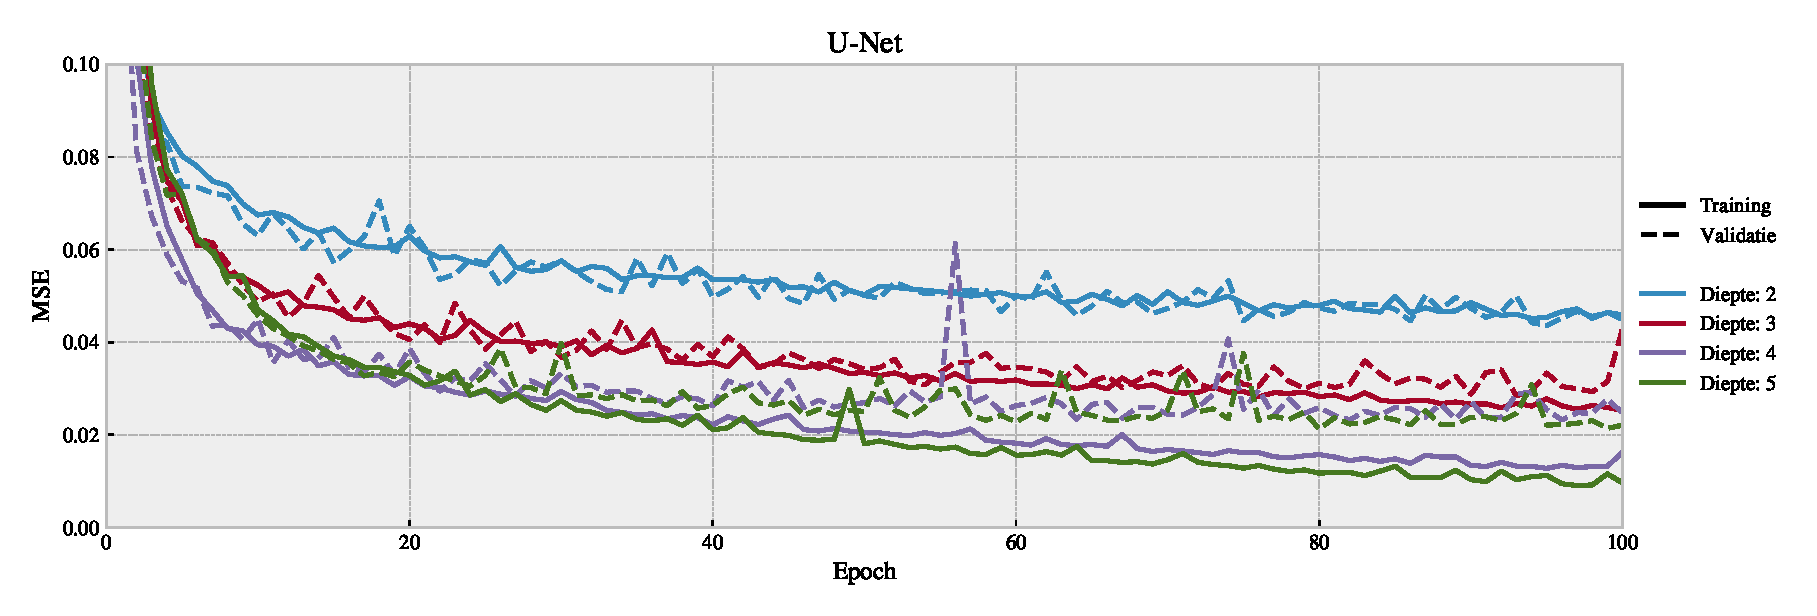
\includegraphics[width=15cm]{images/nets/unet_depth.eps}
	\caption{Resultaten van het U-Net voor verschillende dieptes}
	\label{fig:nets_unet_depth}
\end{figure}

\subsection{MS-D-Net}
Het U-Net is een populaire keuze voor ruisvermindering omdat het zeer goede resultaten levert, maar deze netwerkarchitectuur bevat zeer veel parameters die geoptimaliseerd moeten worden. Zelfs bij een beperkte diepte van het U-Net kon er namelijk al overfitting waargenomen worden. Het Mixed-Scale Dense Network (MS-D-Net) is een relatief recente netwerkarchitectuur op het vlak van ruisvermindering en segmentatie \cite{paper:msdnet}. Dit netwerk vereist minder parameters dan U-Net en zal dus beter convergeren als er slechts een beperkte hoeveelheid trainingsdata beschikbaar is. Door het kleinere aantal parameters is er bovendien meer geheugen beschikbaar om het netwerk ook op grotere afbeeldingen te laten werken. Men combineert een compact (dense) convolutioneel netwerk met verschillende dilaties in elke laag om informatie op verschillende schalen te kunnen gebruiken, dit noemt men Mixed-Scale. Een compact netwerk is een netwerk waarbij de input van een bepaalde laag niet enkel bestaat uit de output van de vorige laag, maar ook de output van alle lagen daarvoor. Dat zorgt ervoor dat de informatie van alle voorgaande lagen beschikbaar is in een bepaalde laag. Er zijn daarom minder parameters nodig in elke laag. Mixed-Scale wijst erop dat in elke laag verschillende convolutiefilters gebruikt worden die elk een andere dilatie hebben en dus elk op een andere schaal naar de input kijken \cite{paper:msdnet}. De dilatie van een convolutielaag is het aantal pixels in de input afbeelding die tussen twee pixels van de convolutiefilter liggen. Dit wordt schematisch weergegeven in figuur \ref{fig:tem_dilations}.
\begin{figure}[h!]
	\centering
	\includegraphics[width=12cm]{images/tem/dilations.jpg}
	\caption{Schematische voorstelling de dilatie van een convolutiefilter, de output van elke laag is beschikbaar voor alle volgende lagen (bron: \cite{fig:dilations})}
	\label{fig:tem_dilations}
\end{figure}
\\ \\
In elke laag heeft het MS-D-Net dus zowel toegang tot contextuele informatie over een groot bereik, als gedetailleerde informatie in een kleine omgeving rondom een bepaalde pixel. Een schematische voorstelling van het MS-D-Net is te zien in figuur \ref{fig:tem_msdnet}. Bijgevolg heeft het MS-D-Net veel minder parameters nodig dan het U-Net (ongeveer 50 maal minder parameters, afhankelijk van het aantal lagen). Aangezien er minder parameters geoptimaliseerd moeten worden, is er voor supervised learning minder trainingsdata nodig \cite{paper:msdnet}.
\begin{figure}[h!]
	\centering
	\includegraphics[width=15cm]{images/tem/msdnet.png}
	\caption{Schematische voorstelling van de MS-D-Net architectuur}
	\label{fig:tem_msdnet}
\end{figure}
\\ \\
Ook bij het MS-D-Net moet de diepte eerst geoptimaliseerd worden. Hier wordt de diepte gegeven door het aantal lagen in het netwerk (in figuur \ref{fig:tem_msdnet} is dit de waarde $N$). Figuur \ref{fig:nets_msdnet_depth} toont de resultaten van het MS-D-Net voor verschillende dieptes. Het is meteen duidelijk dat dit netwerk stabieler is dan het U-Net en geen enkele kenmerken van overfitting toont. Dit kan men zien aan het feit dat de fout bij de validatiedata zeer goed overeenkomt met die van de trainingsdata. Ook dient te worden opgemerkt dat de verschillende dieptes van het MS-D-Net steeds convergeren naar dezelfde MSE. De keuze van de diepte heeft dus nauwelijks invloed op de resultaten. Een dieper netwerk vereist echter wel meer geheugen, waardoor het niet gewenst is om al te diepe netwerken te gebruiken, maar convergeert in dit geval wel sneller. In wat volgt zal MSDNet50 gebruikt worden, omdat dit een goed compromis maakt tussen de convergentiesnelheid en het vereiste geheugen.
\begin{figure}[h!]
	\centering
	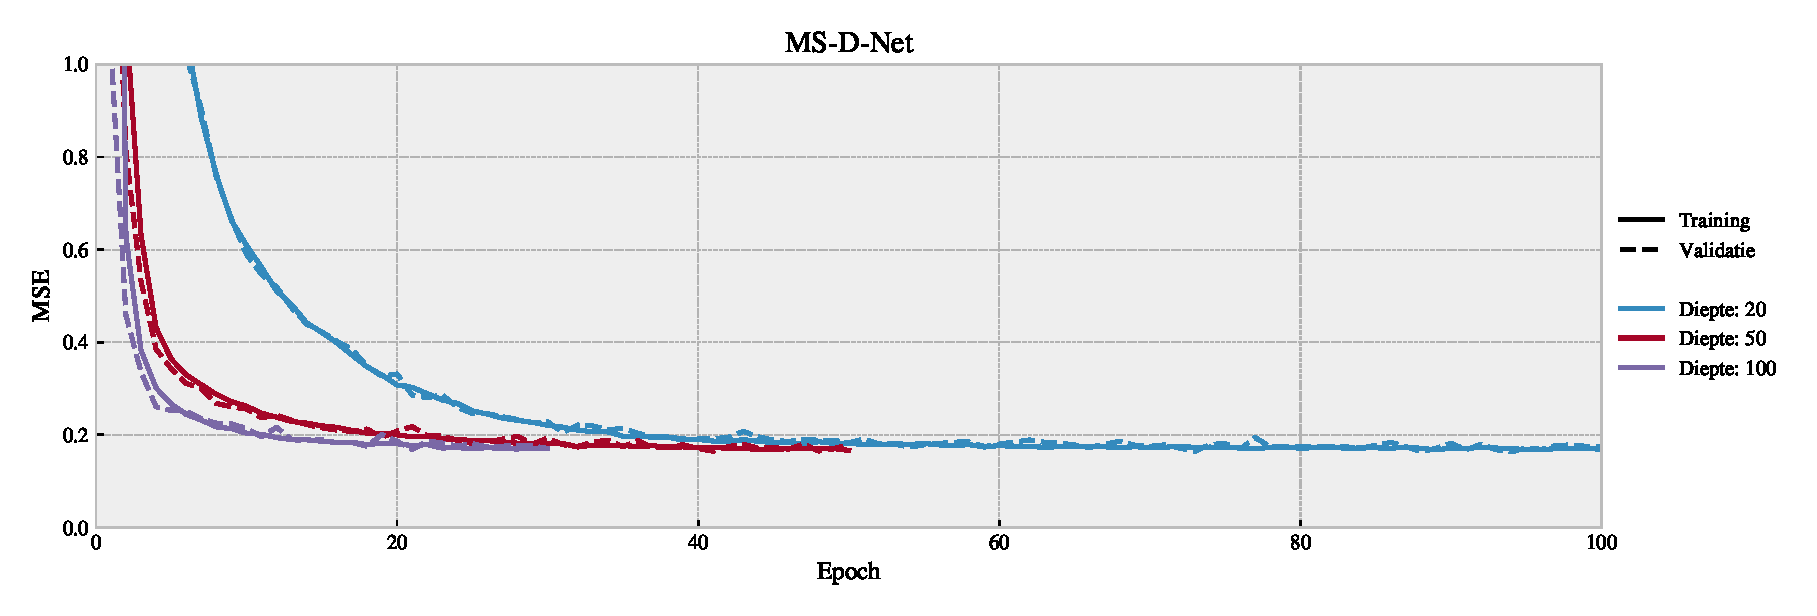
\includegraphics[width=15cm]{images/nets/msdnet_depth.eps}
	\caption{Resultaten van het MS-D-Net voor verschillende dieptes}
	\label{fig:nets_msdnet_depth}
\end{figure}
\\ \\
Vergelijkt men de trainingsresultaten van UNet3 met MSDNet50, dan zou men meteen het U-Net kiezen. Dit haalt namelijk betere resultaten bij het trainen op basis van de gesimuleerde database. Toch zal het MS-D-Net niet buiten beschouwing gehouden worden. Men dient namelijk op te merken dat dit netwerk veel stabieler is tijdens het trainen, geen enkele tekenen van overfitting toont en daarbovenop nog eens specifiek ontworpen is om met minder data goed te convergeren. De verwachting is dus dat het MS-D-Net beter kan veralgemenen naar experimentele data en in dat geval eventueel zelfs de overhand kan halen. Om dat na te gaan worden de resultaten van beide netwerken opnieuw vergeleken aan de hand van de eerder besproken AuAg nanokooi in figuur \ref{fig:nets_net_vis_edx}. Hierbij worden de resultaten ook vergeleken met de best presterende klassieke methode: een gaussische filter. Beide netwerkarchitecturen halen hier resultaten met een hogere PSNR dan het resultaat van de gaussische filter.
\begin{figure}[h!]
	\centering
	\includegraphics[width=15cm]{images/nets/net_vis_edx.png}
	\caption{Visuele resultaten van MSDNet50 in vergelijking met die van UNet3 en een gaussische filter voor een EDX map met als ground-truth een langere meting van hetzelfde object}
	\label{fig:nets_net_vis_edx}
\end{figure}
\\ \\
Het verschil in PSNR tussen de resultaten van de neurale netwerken en het resultaat van de gaussische filter is echter niet groot. Om betere conclusies te kunnen trekken, moet er dus meer data bestudeerd worden. Echter, het is zeer moeilijk om zulke EDX maps te bekomen (i.e. met een langdurige meting als ground-truth). Het zou dus handig zijn indien een HAADF-STEM projectiebeeld met gesimuleerde ruis voldoende representatief is voor EDX maps. Een HAADF-STEM projectiebeeld heeft namelijk een zeer hoge signaal-ruis verhouding en kan als ground-truth gebruikt worden. Een input afbeelding kan dan bekomen worden op dezelfde wijze als bij de gesimuleerde database: door Poisson ruis te simuleren bij deze ground-truth afbeelding. De resultaten van het HAADF-STEM projectiebeeld van de AuAg nanokooi worden getoond in figuur \ref{fig:nets_net_vis_cage}. De resultaten van de verschillende methoden zijn, relatief ten opzichte van elkaar, in goede overeenkomst met die bij de EDX map van deze nanokooi. Dit betekent dat de HAADF-STEM beelden met gesimuleerde ruis inderdaad representatief zijn voor EDX maps.
\begin{figure}[h!]
	\centering
	\includegraphics[width=15cm]{images/nets/net_vis_cage.png}
	\caption{Visuele resultaten van MSDNet50 in vergelijking met die van UNet3 en een gaussische filter voor een HAADF-STEM projectiebeeld van een AuAg nanokooi met gesimuleerde ruis}
	\label{fig:nets_net_vis_cage}
\end{figure}
\\ \\
Het is dus mogelijk om ook de HAADF-STEM beelden van andere nanodeeltjes te bestuderen. Figuur \ref{fig:nets_net_vis_rod} toont de resultaten van een Au@Pt nanostaafje waarvan de Pt schil een dendritische structuur heeft. Dit deeltje is interessant om te beschouwen, want aangezien de gesimuleerde database hiervoor niet representatief is, zullen de resultaten bij dit deeltje aangeven hoe goed de neurale netwerken veralgemenen naar ongekende experimentele data. Hier kan men vaststellen dat het MS-D-Net de hoogste PSNR haalt en dus het best kan veralgemenen.
\begin{figure}[h!]
	\centering
	\includegraphics[width=15cm]{images/nets/net_vis_rod.png}
	\caption{Visuele resultaten van MSDNet50 in vergelijking met die van UNet3 en een gaussische filter voor een HAADF-STEM projectiebeeld van een Au@Pt nanostaafje met gesimuleerde ruis}
	\label{fig:nets_net_vis_rod}
\end{figure}
\\ \\
Bij de resultaten bij deze twee HAADF-STEM beelden wordt het bovendien duidelijk dat het U-Net verschillende details niet goed kan reconstrueren. Bepaalde gebieden in de afbeeldingen worden namelijk te egaal gemaakt bij gebruik van het U-Net. Het MS-D-Net lijkt minder ruis weg te filteren, maar is wel nauwkeuriger en ook de details worden beter hersteld tijdens de ruisvermindering. Om dat beter na te gaan worden de fouten van deze beelden getoond in figuren \ref{fig:nets_error_vis_cage} en \ref{fig:nets_error_vis_rod}. De fout wordt hier berekend als het verschil tussen het resultaat en de ground-truth. Positieve waarden in de fout komen dus overeen met een overschatting van de pixelintensiteit en negatieve waarden met een onderschatting.
\begin{figure}[h!]
	\centering
	\includegraphics[width=15cm]{images/nets/error_vis_cage.png}
	\caption{Visualisatie van de fout op de resultaten van de verschillende ruisverminderingsmethoden voor een HAADF-STEM projectiebeeld van de AuAg nanokooi met gesimuleerde ruis, onder elke afbeelding wordt de foutenmap van die afbeelding getoond, d.i. het verschil tussen die afbeelding en de ground-truth}
	\label{fig:nets_error_vis_cage}
\end{figure}
\begin{figure}[h!]
	\centering
	\includegraphics[width=15cm]{images/nets/error_vis_rod.png}
	\caption{Visualisatie van de fout op de resultaten van de verschillende ruisverminderingsmethoden voor een HAADF-STEM projectiebeeld van het Au@Pt nanostaafje met gesimuleerde ruis, onder elke afbeelding wordt de foutenmap van die afbeelding getoond, d.i. het verschil tussen die afbeelding en de ground-truth}
	\label{fig:nets_error_vis_rod}
\end{figure}
Het belangrijkste om op te letten is de verdeling van de fouten over de afbeeldingen. Bij pure ruis zal dit volledig willekeurig zijn en zijn de fouten dus homogeen verdeeld over het sample. Bij beide figuren kan men zien dat dit bij de foutenmaps van het MS-D-Net inderdaad het geval is. Het MS-D-Net lijkt dus weinig of geen artefacten toe te voegen. Bij zowel de gaussische filter als het U-Net zijn er daarentegen structurele fouten waarneembaar. Bij de nanokooi in figuur \ref{fig:nets_error_vis_cage} kan men zien dat er aan de buitenrand van het nanodeeltje een overschatting aanwezig is na ruisvermindering met een gaussische filter. Dit bevestigt dat deze methode artefacten, i.e. vervaging, toevoegt aan scherpe overgangen. Ook bij de foutenmap van het U-Net bij de nanokooi zijn er structurele fouten te zien, maar dit is meer uitgesproken bij het Au@Pt nanostaafje in figuur \ref{fig:nets_error_vis_rod}. Daar ziet men namelijk zowel bij het U-Net als bij de gaussische filter dat de dendritische structuur van de Pt schil herkenbaar is in de foutenmap. Dit betekent dat deze dendritische structuur niet goed gereconstrueerd werd bij de ruisvermindering.
\\ \\
Er kan dus besloten worden dat zowel het U-Net als het MS-D-Net een gelijkaardige PSNR halen als de best presterende klassieke methode: een gaussische filter. Echter, het MS-D-Net is beter in staat om de structuur van het nanodeeltje nauwkeurig te reconstrueren dan beide andere methoden. Er werden namelijk geen waarneembare artefacten toegevoegd door het MS-D-Net bij de samples die bestudeerd werden.


\chapter{EDX tomografie met neurale netwerken} \label{ch:exp}
In het vorige hoofdstuk toonde ik hoe supervised learning kan leiden tot een betere ruisvermindering dan klassieke technieken. Hier zal ik de getrainde netwerken toepassen op EDX data die gebruikt zal worden voor een tomografische reconstructie. Daarvoor zullen de resultaten eerst kwantitatief besproken worden aan de hand van samples uit de gesimuleerde database. Vervolgens worden er verschillende nanodeeltjes besproken.

\section{Gesimuleerde data} \label{ch:tomo_sim}
Eerst wordt de nauwkeurigheid van de 3D reconstructies kwantitatief besproken door de vijf samples in figuur \ref{fig:data_synthdb} van de gesimuleerde database te onderzoeken. Van deze samples is de ground-truth gekend, waardoor het eenvoudig is om de resultaten kwantitatief te bespreken. Om dat te doen, wordt de vormfout gebruikt. Dit is het percentage aan voxels die fout geclassificeerd zijn en wordt gedefinieerd als het volume van het absolute verschil tussen de gesegmenteerde reconstructie en de ground-truth, relatief ten opzichte van het volume van de ground-truth \cite{paper:shapeerror}:
\[ \text{vormfout} = \frac{\text{Vol}(|\text{reconstructie}-\text{ground-truth}|)}{\text{Vol}(\text{ground-truth})} \cdot 100\% \]
Zowel de reconstructie als de ground-truth zijn daarbij 3D datastructuren met in elke voxel hetzij de waarde nul, hetzij de waarde één. Het volume wordt berekend als het aantal voxels die gelijk zijn aan één.
\\ \\
Om deze samples te bestuderen, werd eerst een tiltreeks gesimuleerd voor elk sample. Om de resultaten vergelijkbaar te maken met die van experimentele EDX data, werd telkens een tiltreeks gesimuleerd met hoeken tussen $-70\degree$ en $70\degree$ in stappen van $10\degree$. Dat levert tiltreeksen op van 15 projectiebeelden. Vervolgens werd Poisson ruis gesimuleerd in die beelden, net zoals bij het creëren van de gesimuleerde database. Op deze beelden met ruis werden de verschillende ruisverminderingsmethoden toegepast (gaussische filter, UNet3 of MSDNet50). Daarna werden de tomografische reconstructies bekomen door gebruik te maken van het EM algoritme met 15 iteraties. Tenslotte werden de gesegmenteerde reconstructies bekomen door de resultaten te segmenteren met de threshold methode van Otsu \cite{paper:otsu}.
\\ \\
Om de resultaten goed te interpreteren, werd ook een reconstructie gemaakt van de tiltreeks zonder ruis. Door de resultaten te vergelijken met deze ``best mogelijke reconstructie'', is het mogelijk om andere effecten, die de nauwkeurigheid van de tomografische reconstructie limiteren, buiten beschouwing te houden. Die andere effecten zijn bijvoorbeeld het gevolg van een klein aantal projectiebeelden te gebruiken of missing wedge artefacten.
\\ \\
De resultaten van de vormfout voor de vijf vermelde objecten worden opgelijst in tabel \ref{tab:tomo_simres}. Daar werd de vormfout berekend door de reconstructie op basis van het ruisvrije signaal als ground-truth te gebruiken. Figuur \ref{fig:tomo_simres} toont een snede door de absolute fout in de voxels van de verschillende reconstructies. Bij elk van deze vijf vormen worden de meest nauwkeurige resultaten bekomen door gebruik te maken van het MS-D-Net. Het U-Net lijkt daarentegen minder geschikt voor gebruik bij tomografie dan het MS-D-Net.
\begin{table}[h!]
	\centering
	\caption{De vormfout van verschillende objecten ten opzichte van de reconstructie op basis van het ruisvrije signaal voor (A) een holle kubus (B) de ribben van kubus (C) een driehoek met afgeronde randen (D) een staafje met afgeronde uiteindes (E) een cilinder}
	\begin{tabular}{|c|ccc|}
		\hline
		Object & gaussische filter & UNet3 & MSDNet50 \\
		\hline
		A & $27.34\%$ & $24.42\%$ & $\textbf{12.87}\%$ \\
		B & $19.52\%$ & $14.72\%$ & $\textbf{ 9.77}\%$ \\
		C & $ 5.34\%$ & $ 4.97\%$ & $\textbf{ 3.14}\%$ \\
		D & $ 1.90\%$ & $ 1.87\%$ & $\textbf{ 1.69}\%$ \\
		E & $ 2.78\%$ & $ 3.61\%$ & $\textbf{ 2.16}\%$ \\
		\hline
	\end{tabular}
	\label{tab:tomo_simres}
\end{table}
\begin{figure}[h!]
	\centering
	\includegraphics[width=15cm]{images/tomo/simulated.png}
	\caption{Een snede door de absolute fout van de gesimuleerde holle kubus bij het gebruik van verschillende ruisverminderingsmethoden. Links staat de ground-truth waartegenover de vormfout berekend werd, d.i. de reconstructie op basis van het ruisvrije signaal}
	\label{fig:tomo_simres}
\end{figure}

\section{Heterogeen Au@Ag nanostaafje} \label{ch:tomo_auag}
Vervolgens wordt een Au@Ag nanostaafje beschouwd waarvan het Au en Ag niet met elkaar vermengd zijn. Bij dit type nanodeeltjes kan men de HAADF-STEM reconstructie segmenteren om de verschillende elementen afzonderlijk te karakteriseren. Die segmentatie zal gebruikt worden om de resultaten van EDX tomografie kwantitatief met elkaar te vergelijken. Voor de metingen werd gebruik gemaakt van een ThermoFisher Tecnai Osiris elektronenmicroscoop, bediend bij een versnelspanning van 200kV. Deze elektronenmicroscoop is uitgerust met een vier-kwadranten Super-X detector die gebruikt werd voor de EDX metingen. Er werd een tiltreeks opgenomen van 15 EDX projectiebeelden met invalshoeken tussen $-70\degree$ en $70\degree$ met intervallen van $10\degree$. Tegelijk werd een tiltreeks van HAADF-STEM projectiebeelden opgenomen met een kleinere intervalafstand van $2\degree$ tussen twee opeenvolgende invalshoeken. Eerst werden de HAADF-STEM projectiebeelden achtereenvolgens met elkaar uitgelijnd door elke twee opeenvolgende beelden met elkaar uit te lijnen aan de hand van hun cross correlatie. De EDX maps werden dan uitgelijnd door de uitlijningsparameters van de HAADF-STEM beelden te hergebruiken.
\\ \\
Figuur \ref{fig:tomo_auag} toont een snede door de resultaten van de tomografische reconstructies van dit nanostaafje, samen met de segmentatie die gebruikt werd om de vormfout te berekenen. Elke segmentatie werd bekomen door middel van Otsu's threshold methode \cite{paper:otsu}. De vormfouten van deze reconstructies worden opgelijst in tabel \ref{tab:tomo_auag}. Bij de reconstructie van Au kan opnieuw besloten worden dat het MS-D-Net de beste resultaten haalt. Bij de reconstructie van Ag wordt de laagste vormfout daarentegen bekomen door gebruik te maken van een gaussische filter. Figuur \ref{fig:tomo_auag} toont echter dat alle EDX reconstructies van Ag veel verschillen van de vorm die bekomen wordt door de HAADF-STEM reconstructie te segmenteren. Er is dus waarschijnlijk nog een andere factor die mee een rol speelt in de foute EDX reconstructie van Ag. Bovendien is de vormfout bij Ag zeer hoog, wat er ook op wijst dat er nog andere oorzaken zijn dan enkel de ruis in de tiltreeks. Mogelijk is dit het gevolg van remstraling veroorzaakt door het Au in de kern, waardoor de hoeveelheid Ag in de kern overschat wordt. Remstraling is straling die uitgezonden wordt wanneer een elektron een versnelling ondergaat, bijvoorbeeld door van richting te veranderen \cite{book:williamscarter}. Hierdoor is de vormfout niet meer accuraat. Kwalitatief kan wel besloten worden dat het Ag bij de resultaten van de neurale netwerken een meer homogene dichtheid heeft dan bij het resultaat na het gebruik van een gaussische filter. Dat is ook wat men verwacht op basis van de informatie in de HAADF-STEM tomografische reconstructie.
\begin{figure}[h!]
	\centering
	\includegraphics[width=15cm]{images/tomo/auag.png}
	\caption{Een snede door de tomografische reconstruties van de EDX tiltreeks na het gebruik van verschillende ruisverminderingsmethoden. Links staat de overeenkomstige snede door de tomografische reconstructie op basis van de HAADF-STEM tiltreeks. Onder elke snede wordt de segmentatie van die snede weergegeven. In de gele gebieden overlappen de segmentaties van Au en Ag met elkaar.}
	\label{fig:tomo_auag}
\end{figure}
\begin{table}[h!]
	\centering
	\caption{De vormfout van de tomografische reconstructies na ruisvermindering toe te passen op de EDX tiltreeks. De segmentatie van de tomografische reconstructie van de HAADF-STEM tiltreeks wordt als ground-truth gebruikt.}
	\begin{tabular}{|c|ccc|}
		\hline
		Element & gaussische filter & UNet3 & MSDNet50 \\
		\hline
		Au & $ 9.38\%$ & $ 8.25\%$ & $\textbf{ 7.57}\%$ \\
		Ag & $\textbf{35.18}\%$ & $36.65\%$ & $48.56\%$ \\
		\hline
	\end{tabular}
	\label{tab:tomo_auag}
\end{table}

\newpage
\section{Legering van een Au@Ag nanostaafje} \label{ch:tomo_alloy}
Als de elementen van een nanodeeltje vermengd zijn, is het niet meer eenvoudig om de elementen afzonderlijk te beschouwen door middel van een segmentatie van de reconstructie van een HAADF-STEM tiltreeks \cite{paper:alloysegmentation}. EDX tomografie is hier dus vereist. In deze sectie zal EDX tomografie besproken worden voor een Au@Ag nanostaafje dat opgewarmd werd voor de metingen. Door die opwarming hebben het goud en zilver een legering gevormd \cite{paper:alloys}. De projectiebeelden voor dit nanodeeltje werden op dezelfde manier bekomen als die van het heterogeen Au@Ag nanostaafje en ook de tomografische reconstructies werden op dezelfde manier berekend.
\\ \\
Een snede en een lijnprofiel door de tomografische reconstructies worden getoond in figuur \ref{fig:tomo_alloy}. Op basis van de reconstructie van de HAADF-STEM tiltreeks kan men verwachten dat zowel de dichtheid van goud als die van zilver homogeen verdeeld zijn en dus weinig veranderen op korte afstanden. Merk wel op dat er ook wat zilver aan de buitenkant van het nanostaafje te vinden is, dit is aangeduid met blauwe pijlen op de figuur. De reconstructie na het gebruik van een gaussische filter toont echter relatief grote variaties op korte afstanden in de dichtheden van beide elementen. Het resultaat na het gebruik van het U-Net is daarentegen zeer egaal. De resultaten van het MS-D-Net zijn minder egaal dan die van de gaussische filter bij dit deeltje. Dit kan verklaard worden door het feit dat de gesimuleerde database representatief is voor dit zeer egale nanodeeltje. Dat verklaart waarom het U-Net in dit geval wel goede resultaten opbrengt en waarom het MS-D-Net minder goede resultaten levert.
\begin{figure}[h!]
	\centering
	\includegraphics[width=15cm]{images/tomo/alloy.png}
	\caption{Een snede door de tomografische reconstructies van de EDX tiltreeks na het gebruik van verschillende ruisverminderingsmethoden. Links staat de overeenkomstige snede door de tomografische reconstructie op basis van de HAADF-STEM tiltreeks. Onder elke snede wordt het lijnprofiel getoond dat door de witte lijn op de snede gaat. Met blauwe pijlen wordt het extra Ag aan de buitenkant van het nanostaafje aangewezen.}
	\label{fig:tomo_alloy}
\end{figure}
\\ \\
Aangezien er een volledige legering van Au en Ag gemaakt is, kan men stellen dat de vorm van zowel Au als Ag gelijk moet zijn aan die van de HAADF-STEM 3D reconstructie. Hier kan dus ook een vormfout bekomen worden door de HAADF-STEM reconstructie als ground-truth te beschouwen. De vormfouten worden opgelijst in tabel \ref{tab:tomo_alloy}. Zoals verwacht werd bij de kwalitatieve analyse, haalt het U-Net hier de laagste vormfouten. De hogere vormfouten bij Ag zijn waarschijnlijk het gevolg van het zilver aan de buitenkant van het nanostaafje. Dat werd namelijk niet herkend in de HAADF-STEM reconstructie.
\begin{table}[h!]
	\centering
	\caption{De vormfout van de tomografische reconstructies na ruisvermindering toe te passen op de EDX tiltreeksen. De segmentatie van de tomografische reconstructie van de HAADF-STEM tiltreeks wordt als ground-truth gebruikt.}
	\begin{tabular}{|c|ccc|}
		\hline
		Element & gaussische filter & UNet3 & MSDNet50 \\
		\hline
		Au & $4.34\%$ & $\textbf{3.48}\%$ & $4.22\%$ \\
		Ag & $5.63\%$ & $\textbf{5.41}\%$ & $6.36\%$ \\
		\hline
	\end{tabular}
	\label{tab:tomo_alloy}
\end{table}

\section{Au@Pt nanostaafje} \label{ch:tomo_aupt}
Tenslotte worden de verschillende ruisverminderingsmethoden nog onderzocht bij een Au@Pt nanostaafje met een ruwe schil. De atoomnummers van deze elementen zijn $Z_{Au}=79$ en $Z_{Pt}=78$. Er is dus geen waarneembaar Z-contrast in de reconstructie op basis van een HAADF-STEM tiltreeks, waardoor EDX tomografie hier vereist is. De opnames van de projectiebeelden en de tomografische reconstructies werden opnieuw op dezelfde manier bekomen als bij het eerste Au@Ag nanostaafje.
\\ \\
Figuur \ref{fig:tomo_aupt} toont een snede door de resultaten van de tomografische reconstructies. Door de kleine details van de Pt schil levert een gaussische filter hier geen goede resultaten. De juiste vorm van de schil kan namelijk niet meer herkend worden. Beide neurale netwerken lijken hier meer accurate resultaten te geven. Voor een betere vergelijking van de resultaten werd er ook een 3D visualisatie gemaakt met behulp van de Amira software. Deze is te zien in figuur \ref{fig:tomo_aupt3d}. Het is meteen duidelijk dat de vorm van de Pt schil niet meer herkenbaar is in het resultaat van de gaussische filter. Het U-Net kan de details van deze schil beter reconstrueren, maar vertoont nog kleine artefacten die niet aanwezig zijn in de HAADF-STEM reconstructie, hiervan zijn er een aantal aangeduid met blauwe cirkels. Het resultaat na ruisvermindering met het MS-D-Net is daarentegen in goede overeenkomst met dat van het HAADF signaal, hoewel het ook niet alle details correct kan reproduceren.
\begin{figure}[h!]
	\centering
	\includegraphics[width=15cm]{images/tomo/aupt.png}
	\caption{Een snede door de tomografische reconstructies van de EDX tiltreeks na het gebruik van verschillende ruisverminderingsmethoden. Links staat de overeenkomstige snede door de tomografische reconstructie op basis van de HAADF-STEM tiltreeks.}
	\label{fig:tomo_aupt}
\end{figure}
\begin{figure}[h!]
	\centering
	\includegraphics[width=15cm]{images/tomo/aupt_3d.png}
	\caption{3D visualisatie van de tomografische reconstructies van het Au@Pt nanostaafje, bij de resultaten van EDX tomografie is Au geel en Pt grijs. Enkele details zijn aangeduid in rode kaders om een goede visuele vergelijking te kunnen maken en enkele artefacten van het U-Net zijn aangeduid in blauwe cirkels.}
	\label{fig:tomo_aupt3d}
\end{figure}

\newpage
\section{Bespreking}
Voor EDX tomografie lijkt het MS-D-Net over het algemeen de beste resultaten te halen. In de kwantitatieve vergelijking van deel \ref{ch:tomo_sim} haalde deze ruisverminderingsmethode consistent de laagste vormfout. Ook bij een kwalitatieve visuele vergelijking tussen de resultaten in deel \ref{ch:tomo_auag} en \ref{ch:tomo_aupt} lijken de resultaten van het MS-D-Net het meest accuraat te zijn. Bij de 3D reconstructie van zilver bij het nanostaafje in deel \ref{ch:tomo_auag} werden de beste kwantitatieve resultaten bekomen met een gaussische filter, maar een kwalitatieve vergelijking van die resultaten leidde tot de conclusie dat ook daar het MS-D-Net de beste resultaten opleverde. Er is dus meer onderzoek nodig alvorens er goede conclusies getrokken kunnen worden. Tenslotte werden de beste resultaten bij het nanostaafje met een legering van Au en Ag (deel \ref{ch:tomo_alloy}) gehaald door gebruik te maken van het U-Net. Bij dit deeltje zijn het Au en Ag namelijk zeer egaal, waardoor de gesimuleerde database hier zeer representatief voor is en het U-Net dus de beste resultaten kon halen.


\chapter{Conclusies} \label{ch:discussion}
In deze thesis werd het potentieel van artificiële neurale netwerken voor ruisvermindering bij EDX maps geëvalueerd. Er werd aangetoond dat deze methoden de ruis in EDX maps nauwkeuriger kunnen reduceren dan klassieke methoden zoals een gaussische filter, totale variatie regularisatie of non-local means. Er werden daarvoor verschillende optimalizatiemethoden en netwerkarchitecturen onderzocht. Wat betreft de optimalizatiemethoden, werd onderzocht of er betere resultaten behaald kunnen worden met self-supervised learning aan de hand van een beperkte experimentele database, ten opzichte van supervised learning met een meer uitgebreide gesimuleerde database. Daar werd gevonden dat supervised learning de beste resultaten levert bij gebruik van de beschikbare data. Ook werd onderzocht welke netwerkarchitectuur het best geschikt is. Enerzijds werd het U-Net beschouwd, dat is een netwerkarchitectuur die frequent gebruikt wordt voor ruisvermindering en segmentatie bij biomedische afbeeldingen. Anderzijds werd een nieuwere netwerkarchitectuur, het MS-D-Net, bestudeerd. Dit netwerk is ontworpen zodat het van minder parameters afhankelijk is en dus ook goed zal convergeren als er minder trainingsdata beschikbaar is. Hieruit bleek dat het U-Net kwantitatief gezien betere resultaten kan halen dan het MS-D-Net, maar dat het ook minder goed kan veralgemenen naar experimentele data. Daardoor gaat de ruisvermindering van het U-Net soms ook gepaard met een verlies van informatie over details in de EDX maps. Het MS-D-Net kan daarentegen beter veralgemenen naar experimentele data, maar kan daardoor ook minder ruis reduceren. Hoe dan ook was er telkens minstens één van beide netwerken in staat om betere resultaten te bekomen dan de klassieke methoden.
\\ \\
Tenslotte werd onderzocht of de ruisvermindering met neurale netwerken het toelaat om een meer nauwkeurige analyse van de 3D chemische samenstelling van nanodeeltjes uit voeren met EDX tomografie. Dit werd eerst op een kwantitatieve manier gedaan. Daarvoor werden een aantal objecten van de gesimuleerde database gebruikt. Van deze objecten werden tiltreeksen gesimuleerd waarop de tomografische reconstructies werden uitgevoerd. Om de resultaten kwantitatief uit te drukken, werd gebruik gemaakt van de vormfout. Voor elk van die objecten werden de beste resultaten bekomen door middel van ruisvermindering met het MS-D-Net. Daarna werden drie verschillende nanostaafjes bestudeerd. Het eerste was een heterogeen Au@Ag nanostaafje. Dit vertoonde voldoende Z-contrast in de 3D reconstructie van de HAADF-STEM tiltreeks. Daarom werd deze reconstructie gesegmenteerd en als ground-truth beschouwd. Op die manier was het mogelijk om ook bij dit deeltje de resultaten op een kwantitatieve manier te vergelijken. Bij de 3D reconstructie van goud werden opnieuw de beste resultaten bekomen met het MS-D-Net. Bij de reconstructie van zilver waren er echter enkele moeilijkheden die waarschijnlijk veroorzaakt zijn door remstraling, met als gevolg dat de vormfout het kleinst was bij gebruik van een gausische filter. Hoe dan ook zorgden deze moeilijkheden ervoor dat de vormfout geen accurate representatie was voor de analyse van dit resultaat. Er is dus meer onderzoek nodig naar de exacte oorzaak van deze moeilijkheden en naar eventuele oplossing hiervoor, alvorens hier correcte conclusies uit te kunnen trekken. Een kwalitatieve en kwantitatieve vergelijking van de resultaten bij een legering van een Au@Ag nanostaafje leidde daarentegen naar een voorkeur voor het U-Net. Tenslotte lijken de resultaten van de neurale netwerken bij een Au@Pt nanostaafje ook beter van die bij het gebruik van een gaussische filter. Daar kon er echter geen kwantitatieve studie uitgevoerd worden. Hoewel de resultaten lijken aan te geven dat het MS-D-Net het best geschikt is voor EDX tomografie, is er dus nog onduidelijkheid over e beste keuze van de netwerkarchitectuur en is meer onderzoek vereist.

\section{Verder onderzoek}
De resultaten van ruisverminderingsmethoden gebaseerd op neurale netwerken zijn veelbelovend, maar de methoden die hier voorgesteld werden, kunnen nog verbeterd worden met meer tijd en middelen. Er werd gebruik gemaakt van supervised learning met een gesimuleerde database om de netwerken te trainen. De database die hiervoor gebruikt werd, is gemaakt op basis van geometrische vormen, maar deze zijn niet volledig representatief voor experimentele EDX data. Hoewel het MS-D-Net goed kan veralgemenen naar experimentele data, was dat slechts in mindere mate mogelijk met het U-Net. Het gebruik van een meer representatieve en uitgebreide trainingsdatabase zal daarom hoogstwaarschijnlijk een positieve invloed hebben op de resultaten van beide netwerkarchitecturen.
\\ \\
Enerzijds werd de kracht van Noise2Noise aangetoond in deel \ref{ch:n2n}. Aangezien het niet mogelijk is om de ground-truth van EDX maps te bekomen, is dit dus de beste trainingsmethode die rechtstreeks gebruik maakt van de experimentele data. Indien er een database gemaakt wordt die geschikt is voor Noise2Noise, dan zal dit ongetwijfeld betere resultaten voortbieden. Anderzijds kan er ook gebruik gemaakt worden van andere middelen. HAADF-STEM projectiebeelden hebben een veel hogere signaal-ruis verhouding dan EDX maps en de intensiteitsverdeling voor deeltjes gemaakt van slechts één element is bij benadering dezelfde als die van een EDX map. Het is dus ook mogelijk om HAADF-STEM projectiebeelden te gebruiken met gesimuleerde ruis voor supervised learning. Daar moet echter in diepte onderzocht worden of de intensiteitsverdeling wel degelijk gelijk is aan die van EDX maps. In HAADF-STEM projectiebeelden is er namelijk ook een achtergrondsignaal waarneembaar dat meestal afkomstig is van het steunrooster van de sample houder.
\\ \\
Bovendien zijn er sommige gevallen, zoals in deel \ref{ch:tomo_alloy}, waar het U-Net de beste resultaten haalt bij EDX tomografie. Dit terwijl het MS-D-Net in bijna alle andere gevallen de overhand lijkt te halen. Een meer uitgebreide studie naar het verschil tussen beide netwerken zal dus kunnen helpen bij het kiezen van de beste netwerkarchitectuur voor elke toepassing.

\section{Besluit}
Er kan besloten worden dat het MS-D-Net gebruikt kan worden voor een nauwkeurige kwantificatie van EDX maps. Dit netwerk haalt dikwijls betere resultaten dan klassieke ruisverminderingsmethoden zoals een gaussische filter. Het nadeel is echter dat de performantie van een neuraal netwerk sterk afhankelijk is van de trainingsdata en trainingsmethoden. Hoewel het MS-D-Net minder data vereist dan andere netwerken, zoals het U-Net, is er nog steeds een uitgebreide trainingsdatabase nodig om de vele parameters van dit een netwerk te optimaliseren. Bovendien is er zeer veel rekenkracht nodig, niet enkel voor dit optimalisatieproces, maar ook voor de toepassing van het netwerk op experimentele data. Afgezien daarvan moet toch benadrukt worden dat dit netwerk kan helpen bij een meer accurate kwantificatie van EDX beelden, en dat een verderzetting van dit onderzoek nog betere resultaten kan opleveren.


\chapter*{Gebruikte afkortingen}
\begin{tabular}{ll}
1D	& Eéndimensionaal \\
2D	& Tweedimensionaal \\
3D	& Driedimensionaal \\
ABF-STEM	& Annular bright-field scanning transmissie elektronenmicroscopie \\
ADF-STEM	& Annular dark-field scanning transmissie elektronenmicroscopie \\
Ag	& Zilver \\
ANN	& Artificiële neurale netwerken \\
Au	& Goud \\
CNN	& Convolutionele neurale netwerken \\
CO	& koolstofmonoxide \\
Cu	& Koper \\
EDX	& Energie-dispersieve X-stralen spectroscopie \\
EM	& Expectation maximization \\
EMAT	& Elektronenmicroscopie voor materiaalonderzoek \\
HAADF-STEM	& High-angle annular dark-field scanning transmissie elektronenmicroscopie \\
MS-D-Net	& Mixed-scale dense network \\
MSE	& Mean-square-error \\
N2N	& Noise2Noise \\
N2V	& Noise2Void \\
NL means	& Non-local means \\
PSNR	& Peak signal-to-noise ratio \\
Pt	& Platinum \\
ReLU	& Rectified linear unit \\
SIRT	& Simultaneous iterative reconstruction technique  \\
STEM	& Scanning transmissie elektronenmicroscopie \\
TEM	& Transmissie elektronenmicroscopie \\
TV	& Totale variatie \\
XEDS	& X-stralen energie-dispersieve spectrometer
\end{tabular}

\bibliography{bibliography}
\bibliographystyle{ieeetr}

\end{document}